\documentclass[11pt]{article}

% include style package preamble
\usepackage{preamble}

% Babel dictionaries, include the languages I use in the paper
\usepackage[main=british,latin]{babel}

%% ----------------------------------------------
%% relative pathnames for figures and tables ----
%% ----------------------------------------------
\graphicspath{ {../../out/graphs/}{./figures/} } % Figures Path
\newcommand*{\TablesPath}{../../out/tables/}
\makeatletter
\newcommand*\ExpandableInput[1]{\@@input#1 }
\makeatother

% High-Res Pictures Option
\DeclareGraphicsExtensions{.pdf, .png}

%----------------------------------------------------------------------------- %
%   External Appendix                                                          %
%----------------------------------------------------------------------------- %

% \usepackage{xr}
% \externaldocument{appendix}
% \usepackage[toc,page]{appendix}

%----------------------------------------------------------------------------- %
%   Working Paper Metadata                                                     %
%----------------------------------------------------------------------------- %

% Citation Aliases (if any)
% 10.5684/soep-core.v35


% Dates
\usepackage[useregional]{datetime2}
% if I want to insert a specific date
\newcommand{\thedate}{\DTMdisplaydate{2017}{02}{21}{-1}}
\newcommand{\monthyeardate}{%
  \DTMenglishmonthname{\@dtm@month} \@dtm@year
}

% Here you can change the date presented in the paper title
% If I want a specific date I put in the date
% \date{This Version: \thedate}
% or if I want the date of today I just insert
\date{This Version: \today}
% or if I want just month and year
% \date{This Version: \monthyeardate}
% or I just remove it
%\date{}

% main title 
\title{Credit Shocks and Populism}
% optional subtitle, leave empty if you dont want it
\renewcommand{\subtitle}{\sc Preliminary Draft: Please do not Circulate}


\author{
    {Nicolò~Fraccaroli} \\
    William R. Rhodes Center\\
    for International Economics and Finance\\
    Brown University\\
    \href{mailto:nicolo_fraccaroli@brown.edu}{\texttt{nicolo\_fraccaroli@brown.edu}} \\
    %% examples of more authors
    \And
    {Alessandro~Pizzigolotto} \\
    Department of Economics and FAIR-CELE\\
    Norwegian School of Economics (NHH)\\
    %Santa Narimana, Levand \\
    \href{mailto:alessandro.pizzigolotto@nhh.no}{\texttt{alessandro.pizzigolotto@nhh.no}} \\
    %\AND
    %{Elias D.~Striatum}\thanks{Department of Electrical Engineering, Santa Narimana, Levand, \texttt{stariate@ee.mount-sheikh.edu}.} \\
    %Department of Electrical Engineering\\
    %Mount-Sheikh University\\
    %Santa Narimana, Levand \\
    %\texttt{stariate@ee.mount-sheikh.edu} \\
    %% \And
    %% Coauthor \\
    %% Affiliation \\
    %% Address \\
    %% \texttt{email} \\
    %% \And
    %% Coauthor \\
    %% Affiliation \\
    %% Address \\
    %% \texttt{email} \\
}

%%% Add PDF metadata to help others organize their library
%%% Once the PDF is generated, you can check the metadata with
%%% $ pdfinfo template.pdf
\hypersetup{
    pdftitle={Credit Shock and Populism},
    pdfsubject={Political Economy, Great Financial Crisis, Credit Shock, Political Finance, Credit Risk, Electoral Preferences},
    pdfauthor={Nicolò~Fraccaroli, Alessandro~Pizzigolotto},
    pdfkeywords={milestones, populism, credit, commerzbank, finance, crisis},
}

%----------------------------------------------------------------------------- %
%   TITLE PAGE                                                                 %
%----------------------------------------------------------------------------- %

\begin{document}
\maketitle

\renewcommand{\thefootnote}{\arabic{footnote}}
\setcounter{footnote}{0} 


%----------------------------------------------------------------------------- %
%   ABSTRACT                                                                   %
%----------------------------------------------------------------------------- %

% \begin{abstract}
% \noindent\lipsum[1]
% \end{abstract}
% {\textbf{JEL Classification:} P16; G21; D72; E51} \\
% {\textbf{Keywords:} Monetary Policy, Income Inequality, Structural VAR, Average Propensity of Consume}

% \clearpage\newpage

%----------------------------------------------------------------------------- %
%  TABLE OF CONTENTS                                                           %
%----------------------------------------------------------------------------- %

% \tableofcontents
% \listoftodos

% \clearpage\newpage

%----------------------------------------------------------------------------- %
%   DOCUMENT BODY                                                              %
%----------------------------------------------------------------------------- %

% Introduction
%-----------------------------------------------------------------------------

\begin{figure}[htbp!]
    \centering
    \caption{The Lending Stock of German Banks: Commerzbank vs. All}\label{fig:banks_lending_stock}
    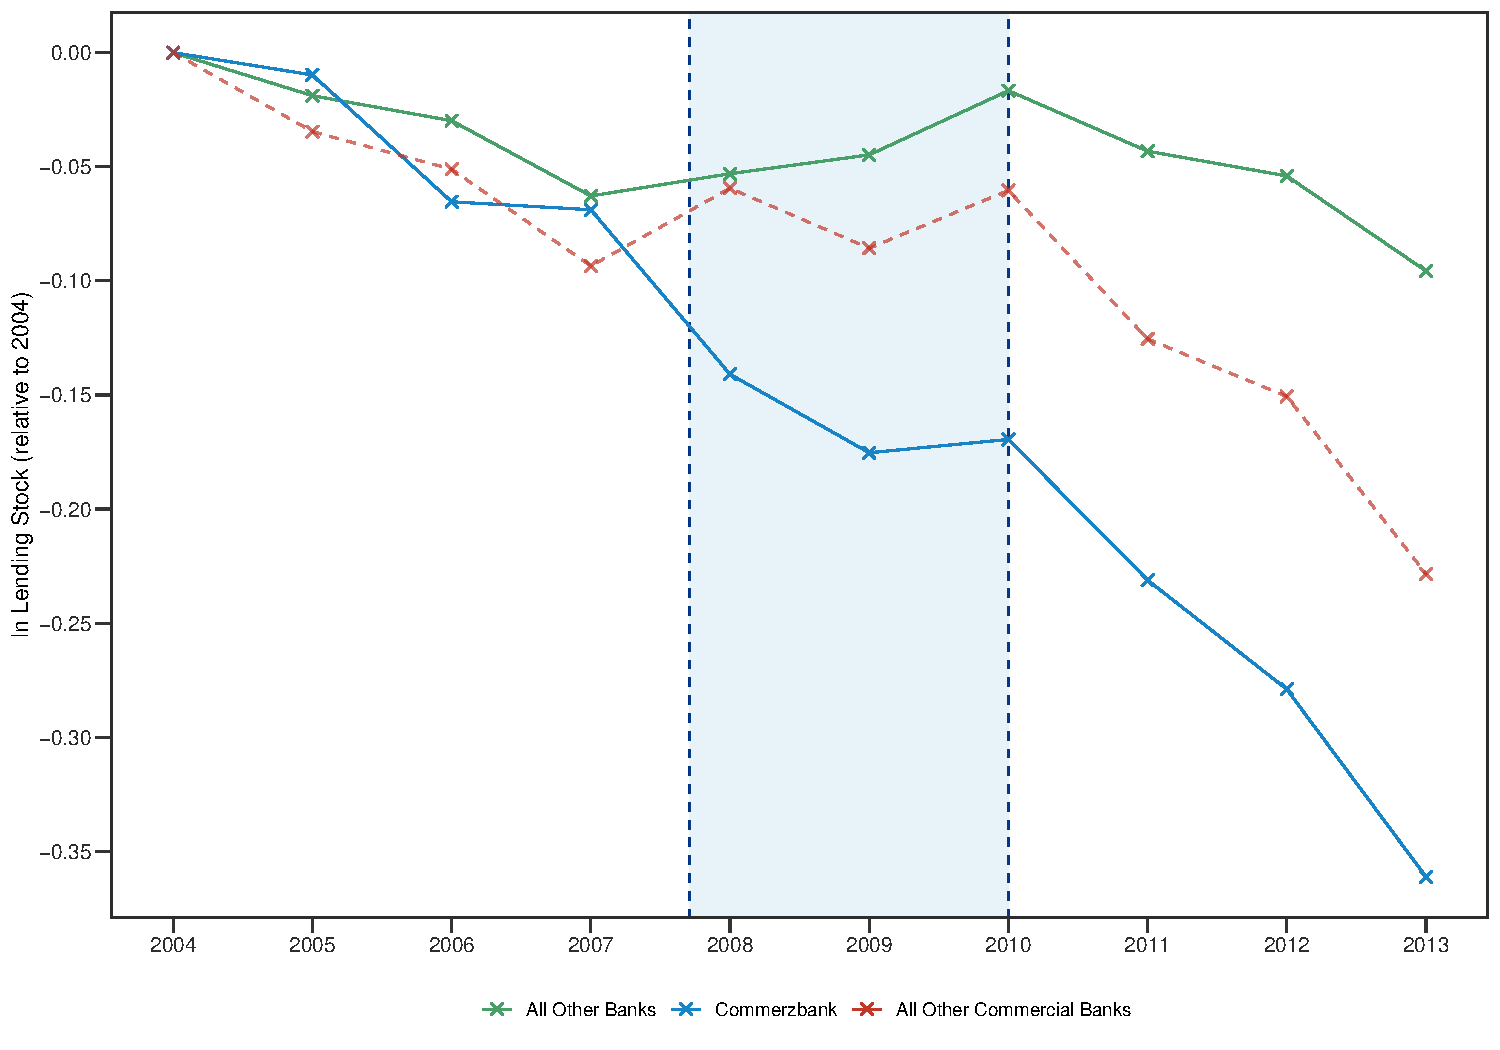
\includegraphics[width=1\linewidth]{shock/huber_lending_cut}
    \begin{tablenotes}
        \footnotesize
        \item \textbf{Notes:} The graph shows the $\ln$ lending stock to German non-financial customers, relative to the year 2004, in 2010 billions of euros. Data for Commerzbank include lending by branches of Commerzbank and Dresdner bank, summing their lending stock for the years before 2009 Dresdner Bank's take-over, using information from the annual reports. For all other banks, data come from Deutsche Bundesbank on German banks and subtract lending by Commerzbank. For all other commercial banks, lending stock of Commerzbank, the savings banks, the Landesbanken, and the cooperative banks is removed. Replication from data and calculation in \citet{bib:huber2018}. We thank Kilian Huber for kindly share the information with us.
    \end{tablenotes} 
\end{figure}

\begin{table}[H]
    \centering
    \caption{Summary Statistics}
    \label{tab:summary_statistics}
    \resizebox{\textwidth}{!}{%
        \ExpandableInput{\TablesPath/descriptives/summary_table}
    }%
    \caption*{\footnotesize \textbf{Notes:} This table shows ... \hl{XXX}.}
\end{table}

\begin{table}[H]
    \centering
    \caption{The Effect of the Credit Shock on Political Support: Difference-in-Differences Results}
    \label{tab:reduced_form_political_support_baseline}
    \def\sym#1{\ifmmode^{#1}\else\(^{#1}\)\fi}
    \resizebox{\textwidth}{!}{%
        \ExpandableInput{\TablesPath/baseline/rf_ps_cbk_past_mean}
    }%
    \caption*{\footnotesize \textbf{Notes:}~This table shows ... \hl{XXX}.}
\end{table}

\begin{table}[H]
    \centering
    \caption{The Effect of the Credit Shock on Intention to Vote for a Populist Party: Difference-in-Differences Results}
    \label{tab:reduced_form_populist_party_baseline}
    \def\sym#1{\ifmmode^{#1}\else\(^{#1}\)\fi}
    \resizebox{\textwidth}{!}{%
        \ExpandableInput{\TablesPath/baseline/rf_pp_cbk_past_mean}
    }%
    \caption*{\footnotesize \textbf{Notes:}~This table shows ... \hl{XXX}.}
\end{table}

\begin{table}[H]
    \centering
    \caption{The Effect of the Credit Shock on Political Support: Difference-in-Differences with Binary Treatment}
    \label{tab:reduced_form_political_support_dummies}
    \def\sym#1{\ifmmode^{#1}\else\(^{#1}\)\fi}
    \resizebox{\textwidth}{!}{%
        \ExpandableInput{\TablesPath/baseline/rf_ps_cbk_past_mean_dummies}
    }%
    \caption*{\footnotesize \textbf{Notes:}~This table shows ... \hl{XXX}.}
\end{table}

\begin{table}[H]
    \centering
    \caption{The Effect of the Credit Shock on Intention to Vote for a Populist Party: Difference-in-Differences with Binary Treatment}
    \label{tab:reduced_form_populist_party_dummies}
    \def\sym#1{\ifmmode^{#1}\else\(^{#1}\)\fi}
    \resizebox{\textwidth}{!}{%
        \ExpandableInput{\TablesPath/baseline/rf_pp_cbk_past_mean_dummies}
    }%
    \caption*{\footnotesize \textbf{Notes:}~This table shows ... \hl{XXX}.}
\end{table}


%%%%%%%%% EVENT STUDY PLOTS WITH DIFFERENT CUTOFFS

\begin{figure}[htbp!]
    \centering
    \caption{Event Study Plot: Political Support - Cutoff Median (without individual FE)}\label{fig:dynamic_did_cbk_past_mean_ps_p50_noife}
    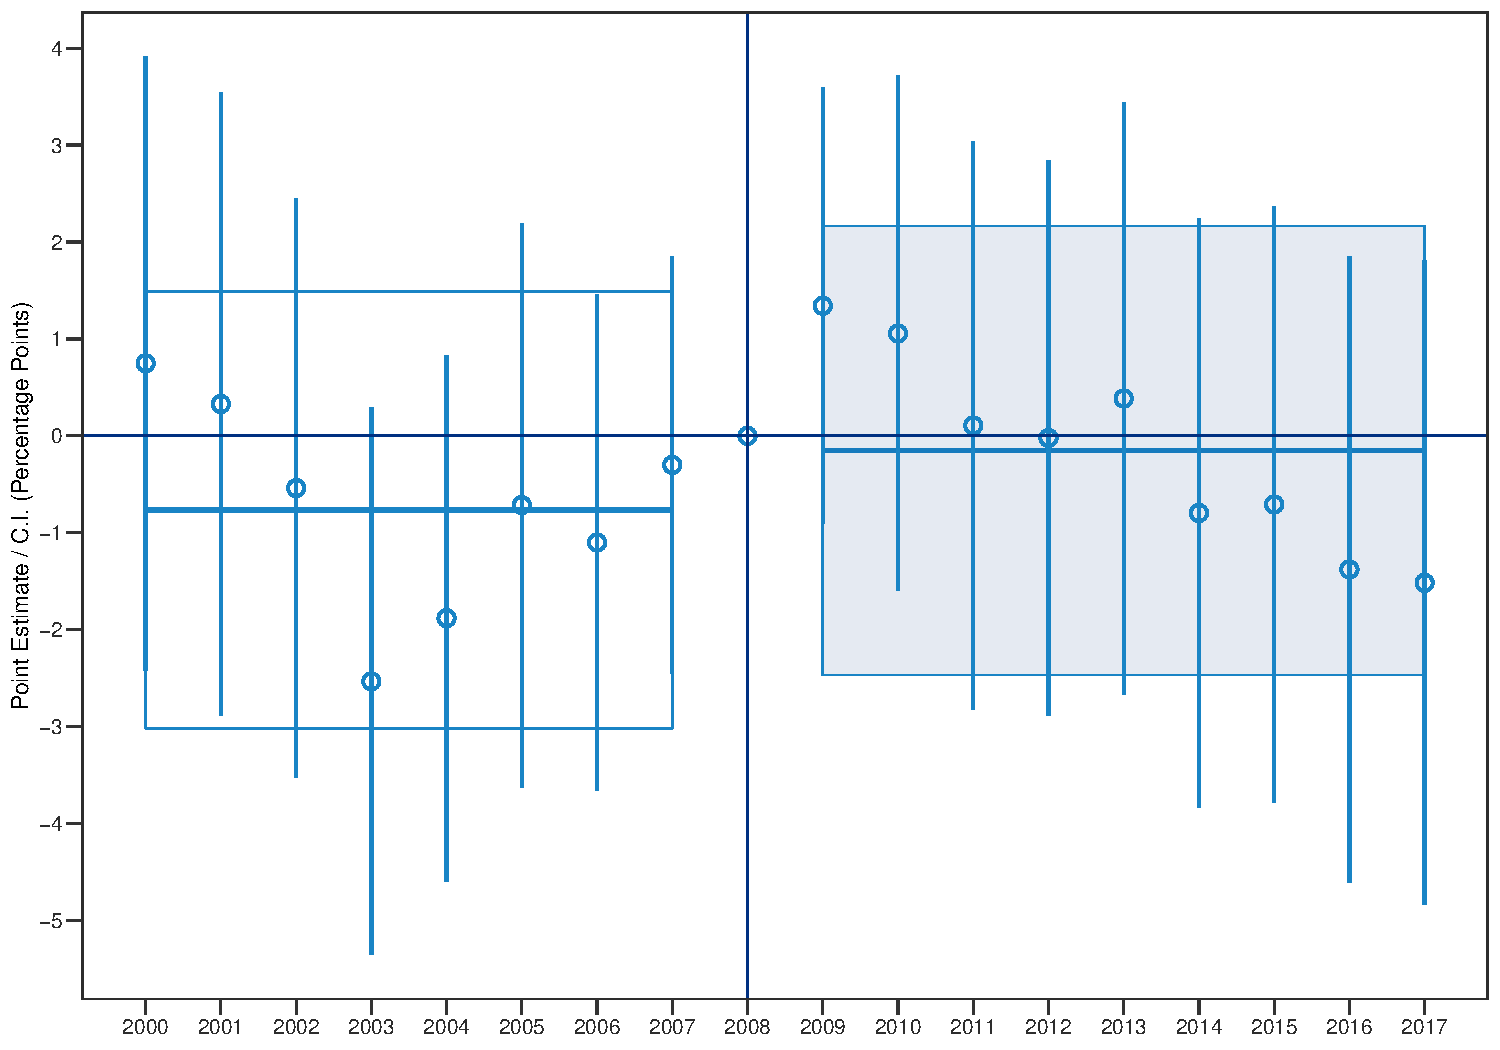
\includegraphics[width=1\linewidth]{events/dynamic_did_cbk_past_mean_ps_p50_noife}
    \begin{tablenotes}
        \footnotesize
        \item \textbf{Notes:}~This table shows ... \hl{XXX}.
    \end{tablenotes} 
\end{figure}

\begin{figure}[htbp!]
    \centering
    \caption{Event Study Plot: Political Support - Cutoff Median (with individual FE)}\label{fig:dynamic_did_cbk_past_mean_ps_p50_ife}
    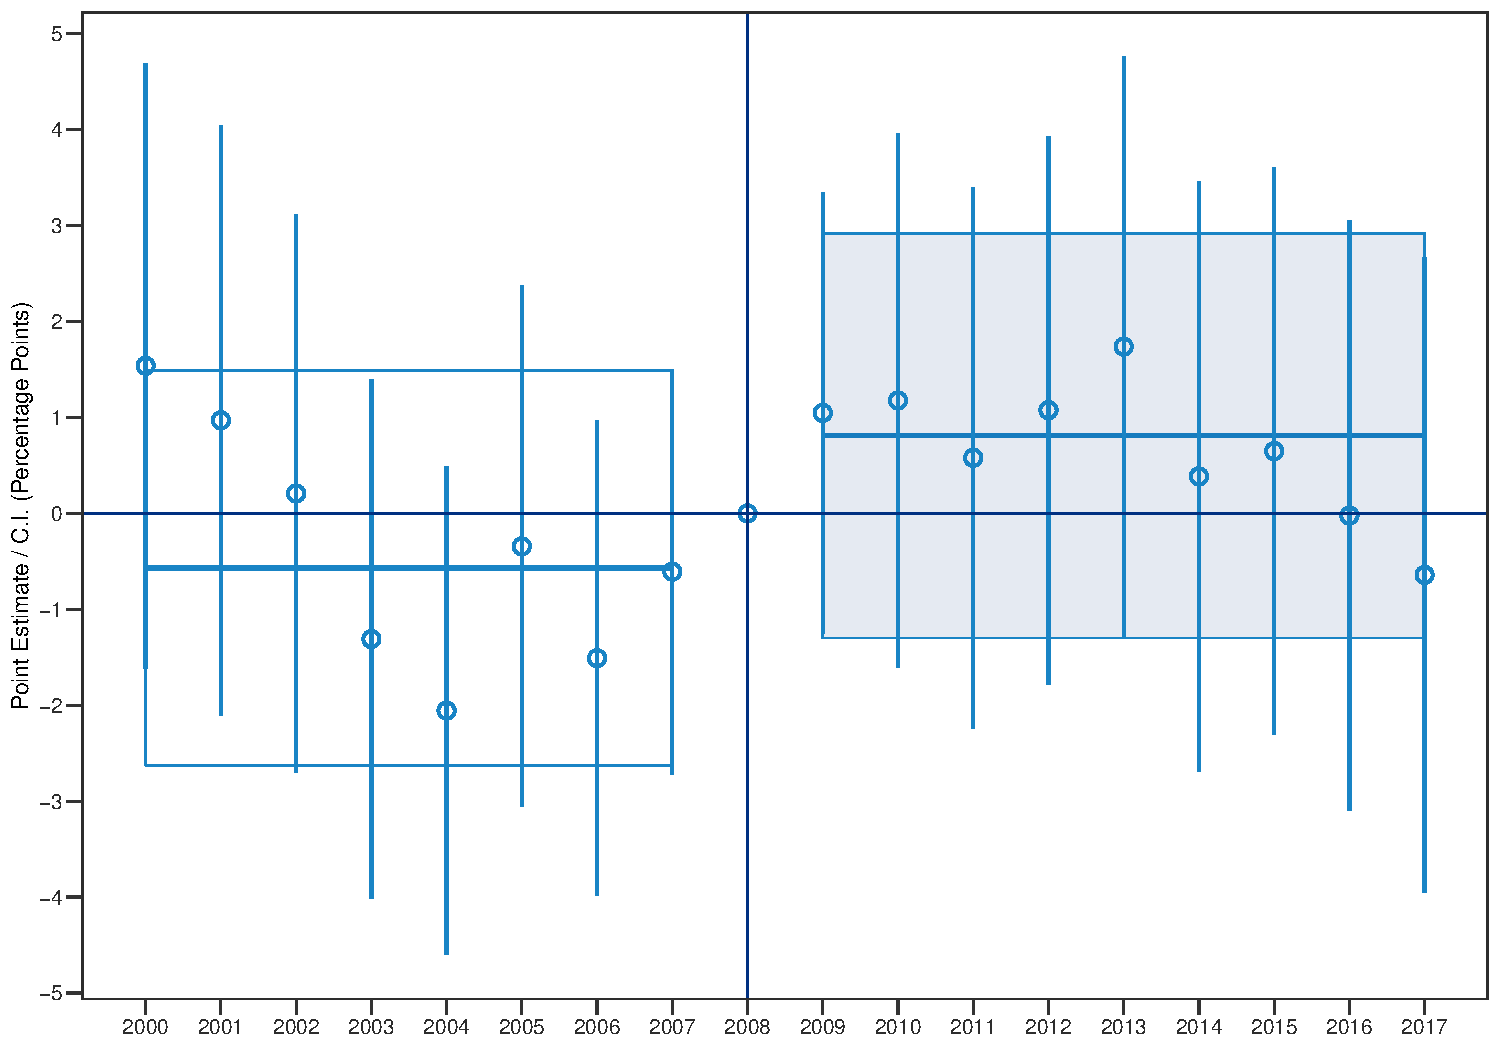
\includegraphics[width=1\linewidth]{events/dynamic_did_cbk_past_mean_ps_p50_ife}
    \begin{tablenotes}
        \footnotesize
        \item \textbf{Notes:}~This table shows ... \hl{XXX}.
    \end{tablenotes} 
\end{figure}

\begin{figure}[htbp!]
    \centering
    \caption{Event Study Plot: Populist Party - Cutoff Median (without individual FE)}\label{fig:dynamic_did_cbk_past_mean_pp_p50_noife}
    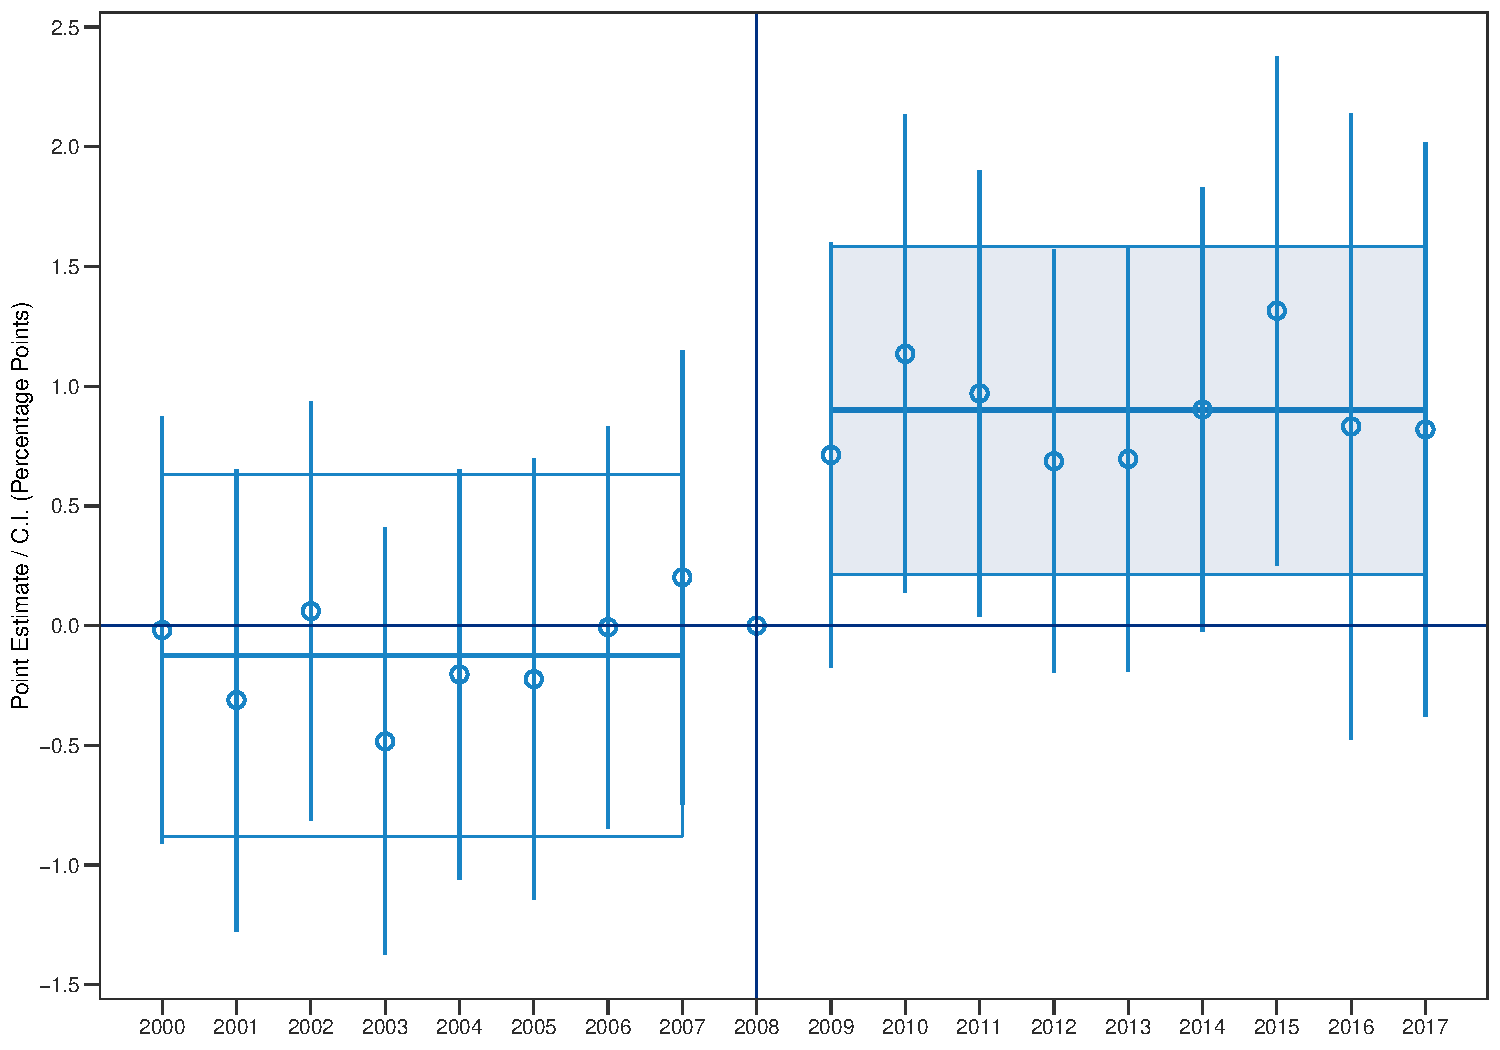
\includegraphics[width=1\linewidth]{events/dynamic_did_cbk_past_mean_pp_p50_noife}
    \begin{tablenotes}
        \footnotesize
        \item \textbf{Notes:}~This table shows ... \hl{XXX}.
    \end{tablenotes} 
\end{figure}

\begin{figure}[htbp!]
    \centering
    \caption{Event Study Plot: Populist Party - Cutoff Median (with individual FE)}\label{fig:dynamic_did_cbk_past_mean_pp_p50_ife}
    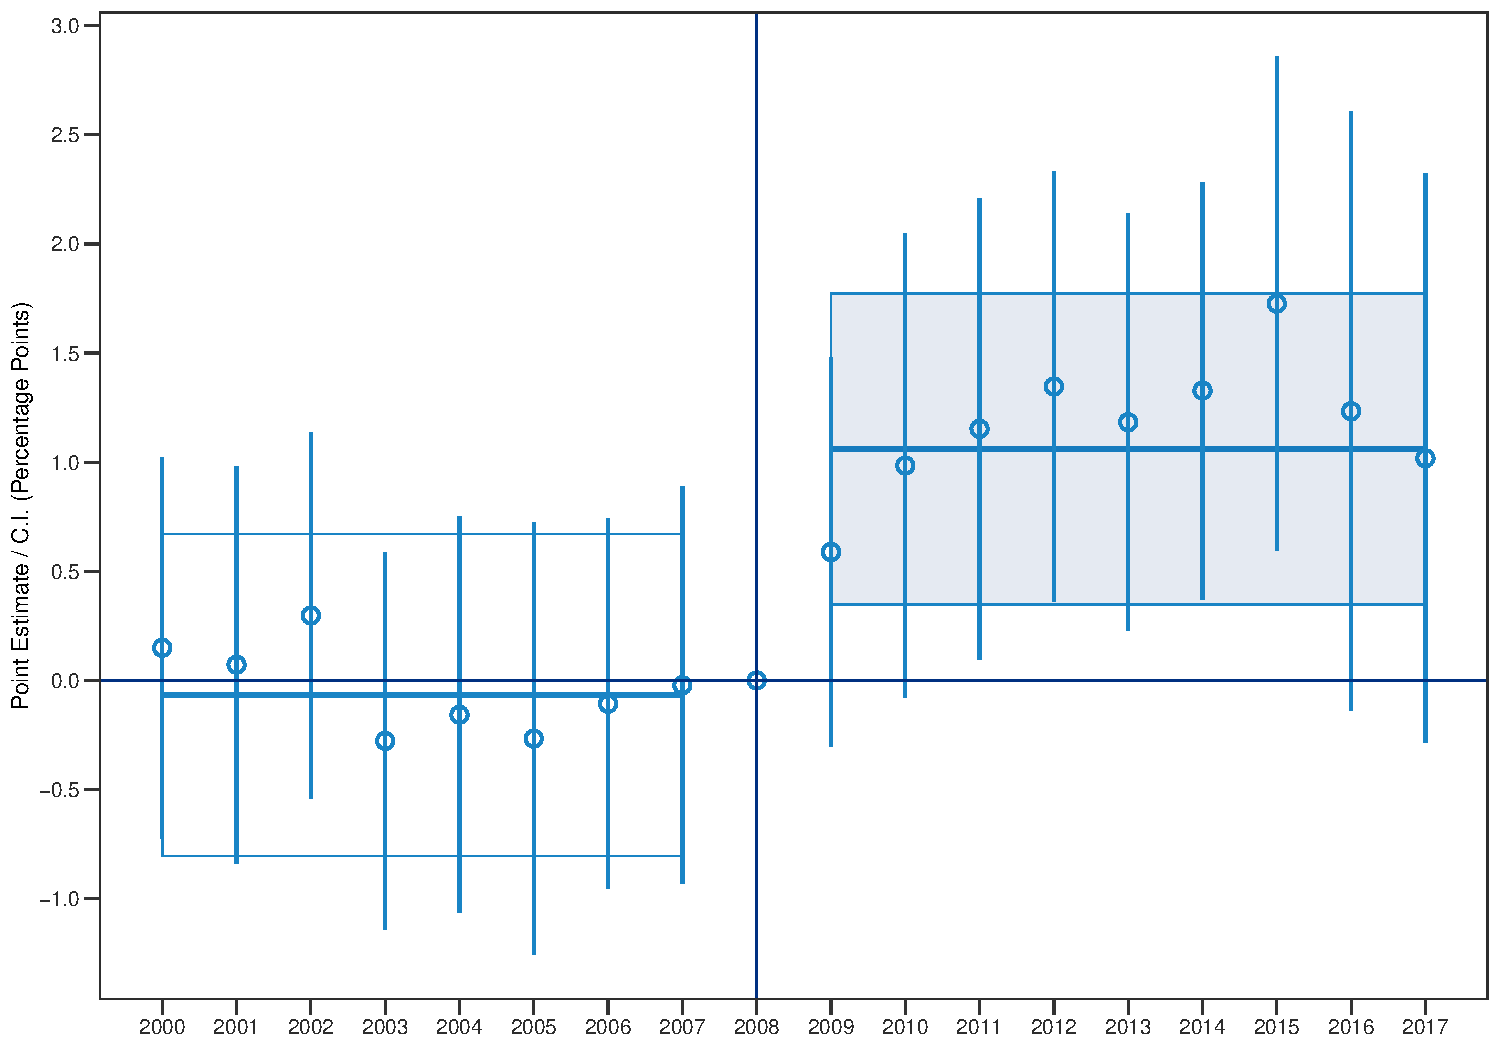
\includegraphics[width=1\linewidth]{events/dynamic_did_cbk_past_mean_pp_p50_ife}
    \begin{tablenotes}
        \footnotesize
        \item \textbf{Notes:}~This table shows ... \hl{XXX}.
    \end{tablenotes} 
\end{figure}

\begin{figure}[htbp!]
    \centering
    \caption{Event Study Plot: Political Support - Cutoff $75^{th}$ Percentile (without individual FE)}\label{fig:dynamic_did_cbk_past_mean_ps_p75_noife}
    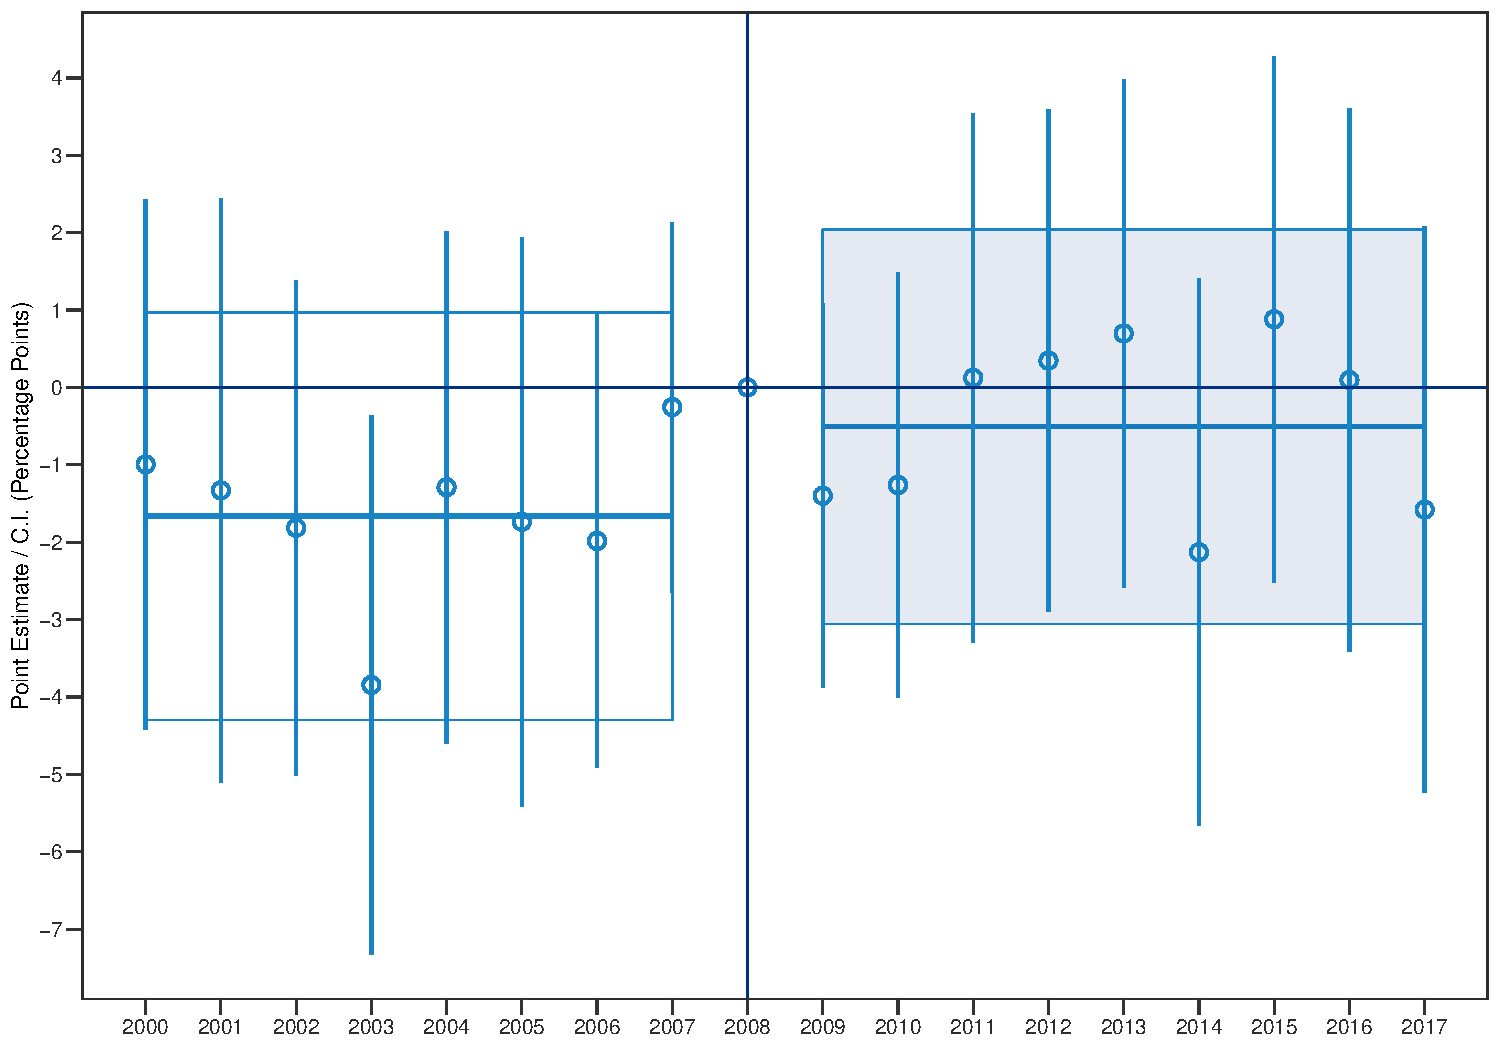
\includegraphics[width=1\linewidth]{events/dynamic_did_cbk_past_mean_ps_p75_noife}
    \begin{tablenotes}
        \footnotesize
        \item \textbf{Notes:}~This table shows ... \hl{XXX}.
    \end{tablenotes} 
\end{figure}

\begin{figure}[htbp!]
    \centering
    \caption{Event Study Plot: Political Support - Cutoff $75^{th}$ Percentile (with individual FE)}\label{fig:dynamic_did_cbk_past_mean_ps_p75_ife}
    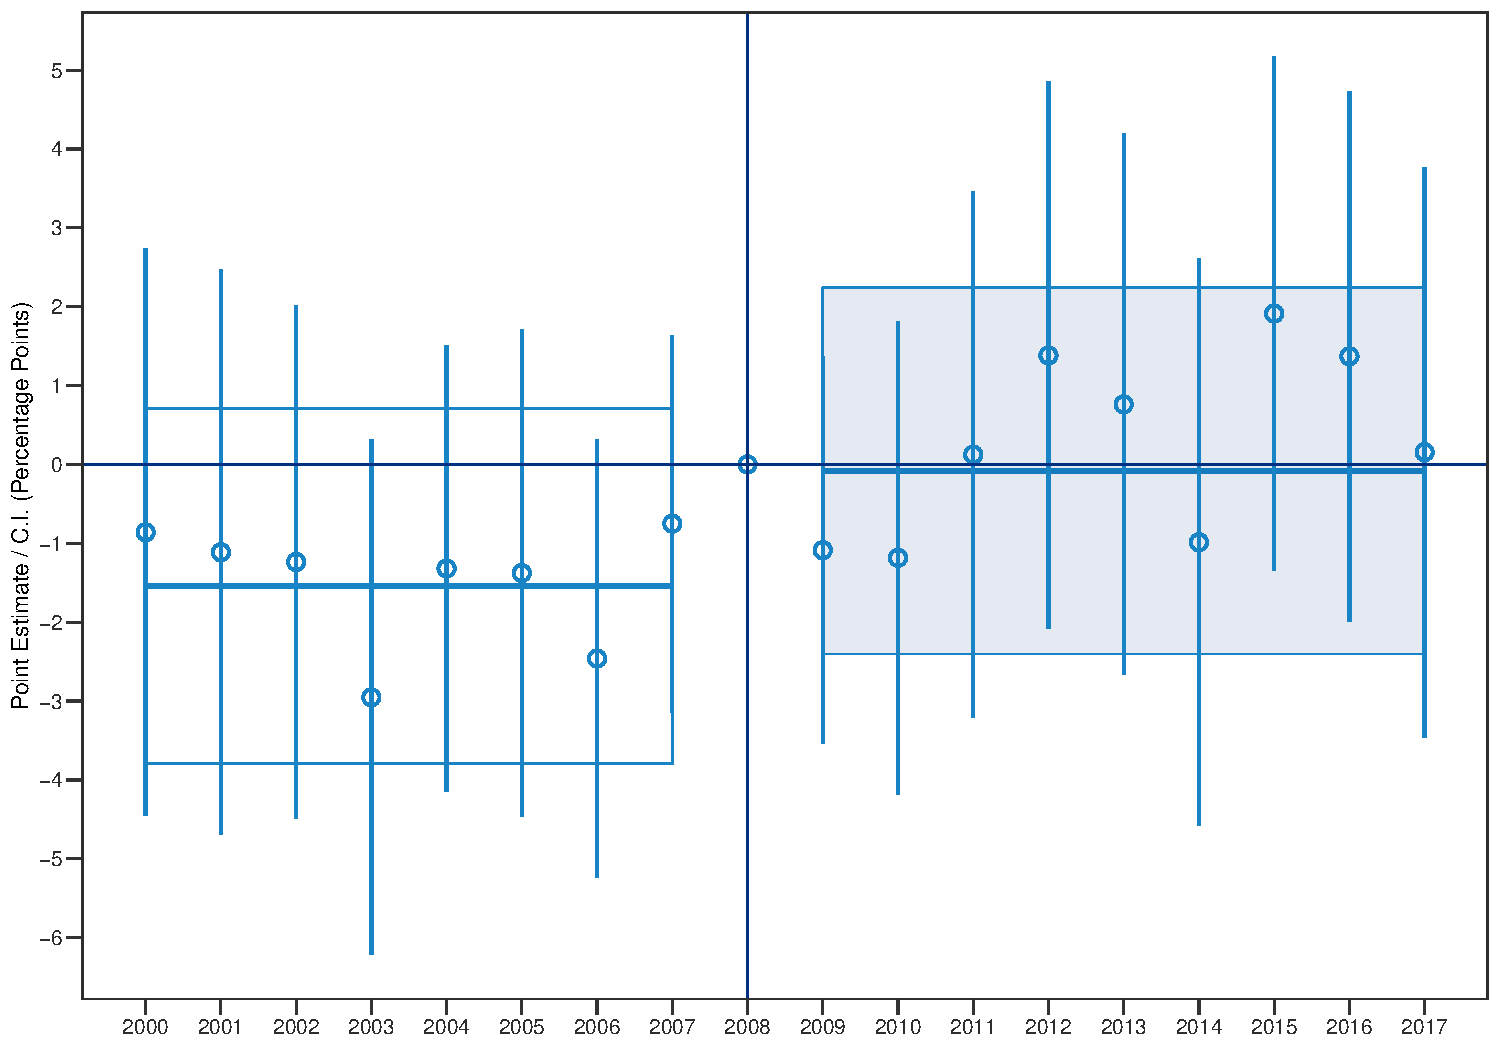
\includegraphics[width=1\linewidth]{events/dynamic_did_cbk_past_mean_ps_p75_ife}
    \begin{tablenotes}
        \footnotesize
        \item \textbf{Notes:}~This table shows ... \hl{XXX}.
    \end{tablenotes} 
\end{figure}

\begin{figure}[htbp!]
    \centering
    \caption{Event Study Plot: Populist Party - Cutoff $75^{th}$ Percentile (without individual FE)}\label{fig:dynamic_did_cbk_past_mean_pp_p75_noife}
    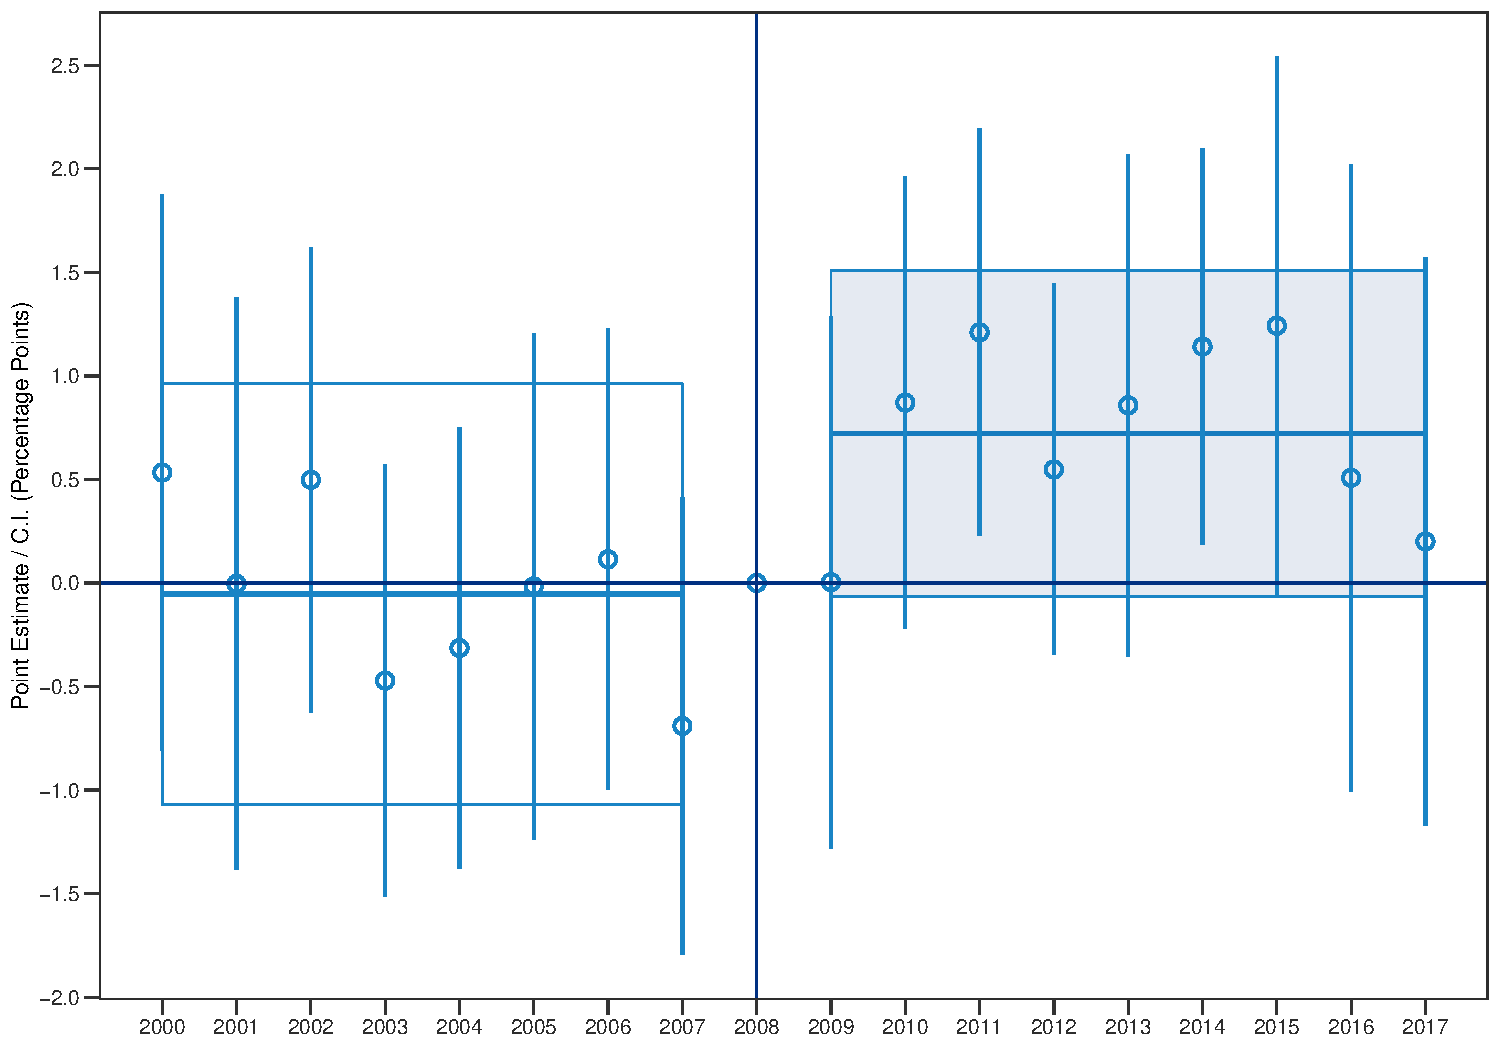
\includegraphics[width=1\linewidth]{events/dynamic_did_cbk_past_mean_pp_p75_noife}
    \begin{tablenotes}
        \footnotesize
        \item \textbf{Notes:}~This table shows ... \hl{XXX}.
    \end{tablenotes} 
\end{figure}

\begin{figure}[htbp!]
    \centering
    \caption{Event Study Plot: Populist Party - Cutoff $75^{th}$ Percentile (with individual FE)}\label{fig:dynamic_did_cbk_past_mean_pp_p75_ife}
    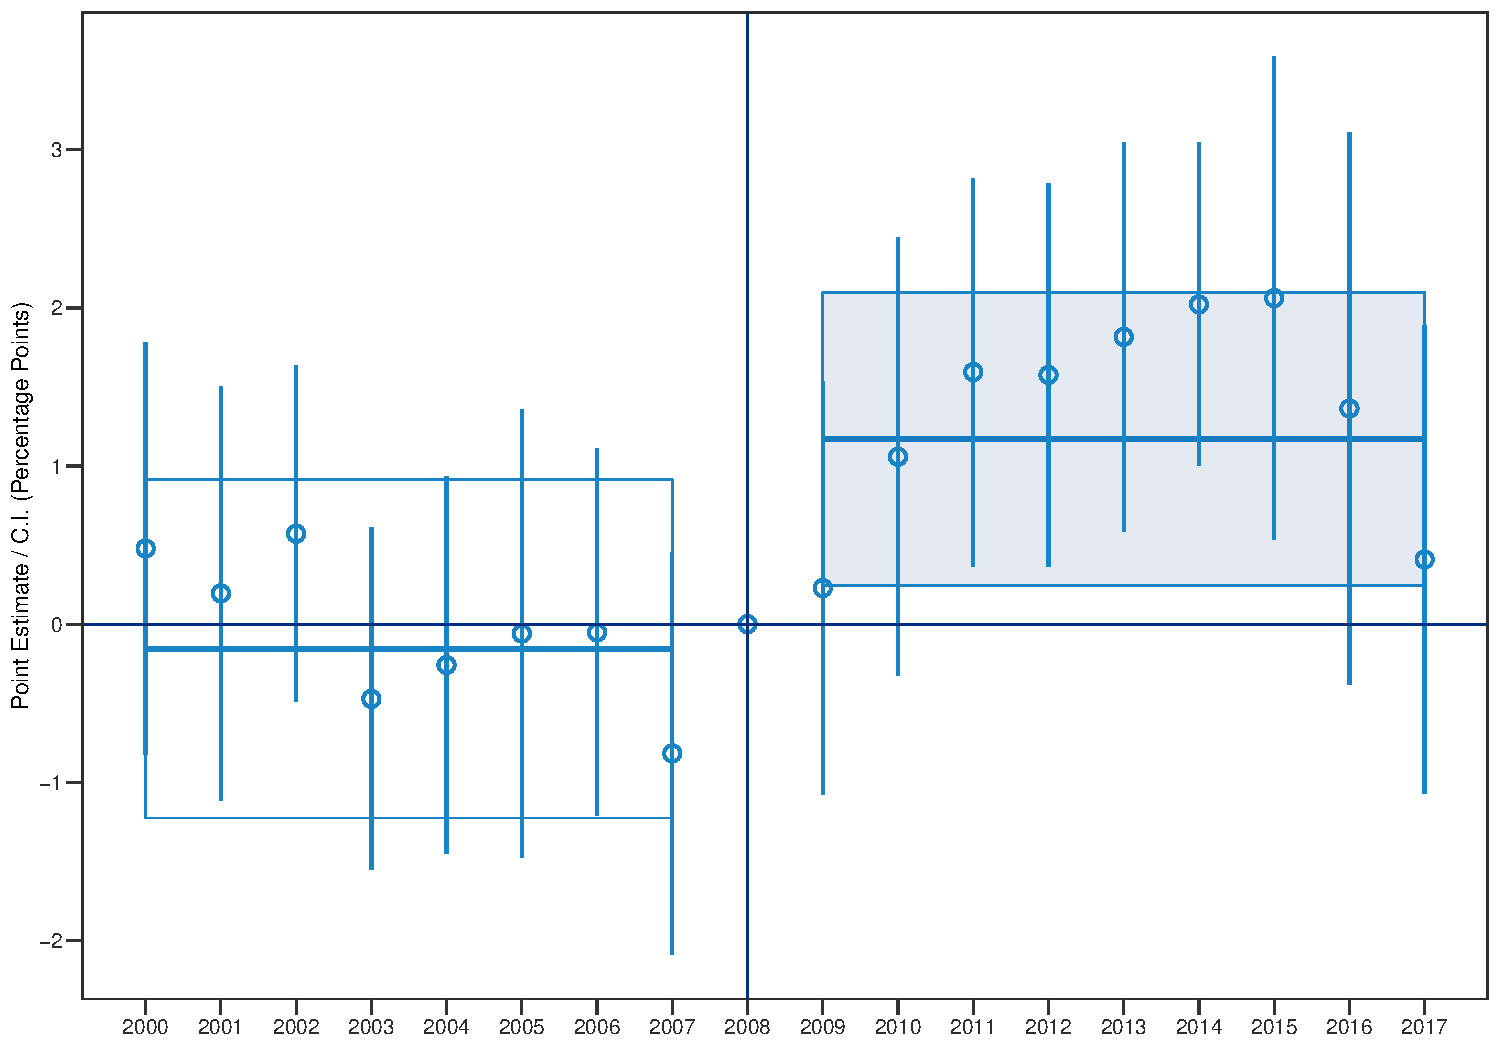
\includegraphics[width=1\linewidth]{events/dynamic_did_cbk_past_mean_pp_p75_ife}
    \begin{tablenotes}
        \footnotesize
        \item \textbf{Notes:}~This table shows ... \hl{XXX}.
    \end{tablenotes} 
\end{figure}


\begin{figure}[htbp!]
    \centering
    \caption{Event Study Plot: Political Support - Cutoff $90^{th}$ Percentile (without individual FE)}\label{fig:dynamic_did_cbk_past_mean_ps_p90_noife}
    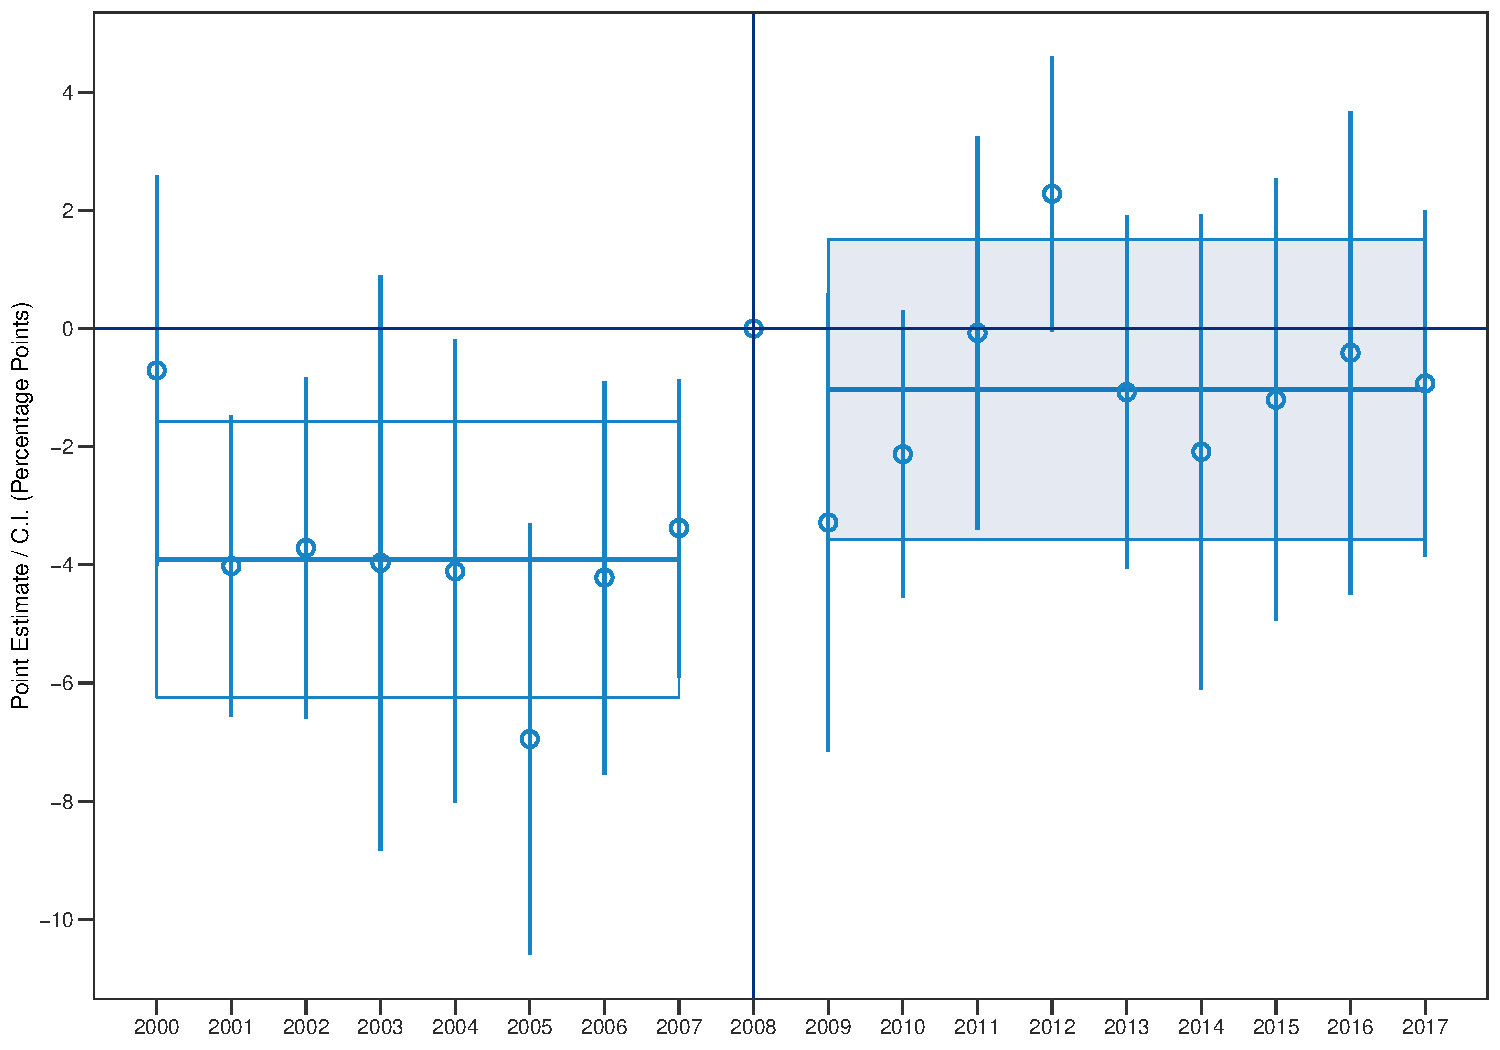
\includegraphics[width=1\linewidth]{events/dynamic_did_cbk_past_mean_ps_p90_noife}
    \begin{tablenotes}
        \footnotesize
        \item \textbf{Notes:}~This table shows ... \hl{XXX}.
    \end{tablenotes} 
\end{figure}

\begin{figure}[htbp!]
    \centering
    \caption{Event Study Plot: Political Support - Cutoff $90^{th}$ Percentile (with individual FE)}\label{fig:dynamic_did_cbk_past_mean_ps_p90_ife}
    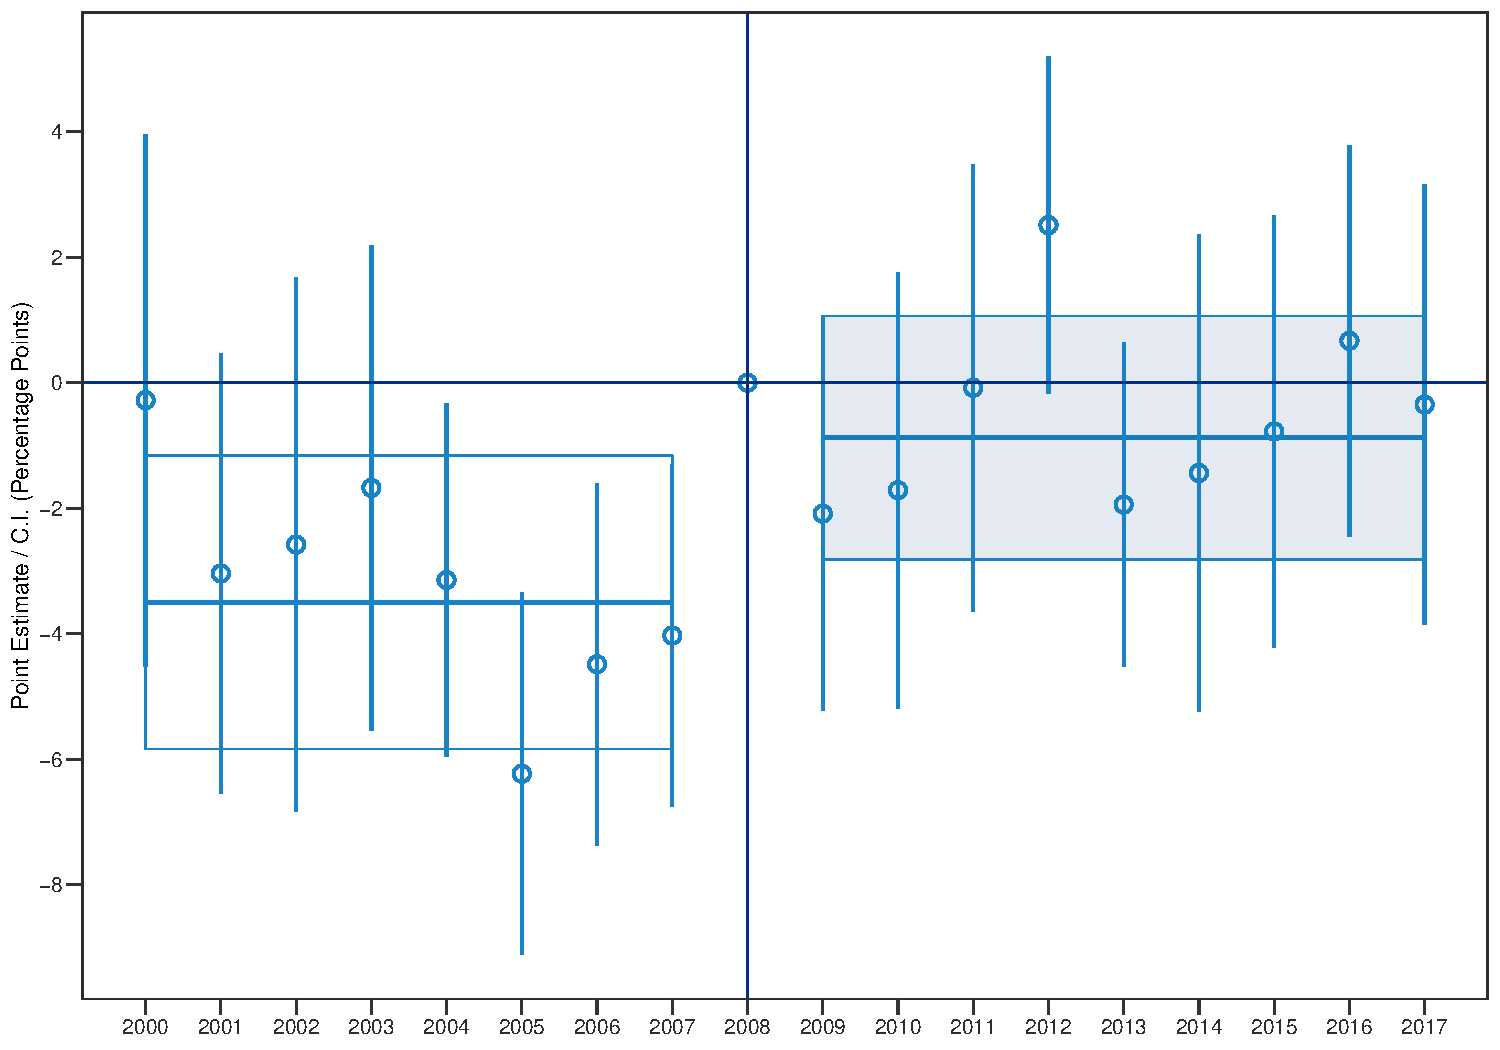
\includegraphics[width=1\linewidth]{events/dynamic_did_cbk_past_mean_ps_p90_ife}
    \begin{tablenotes}
        \footnotesize
        \item \textbf{Notes:}~This table shows ... \hl{XXX}.
    \end{tablenotes} 
\end{figure}

\begin{figure}[htbp!]
    \centering
    \caption{Event Study Plot: Populist Party - Cutoff $90^{th}$ Percentile (without individual FE)}\label{fig:dynamic_did_cbk_past_mean_pp_p90_noife}
    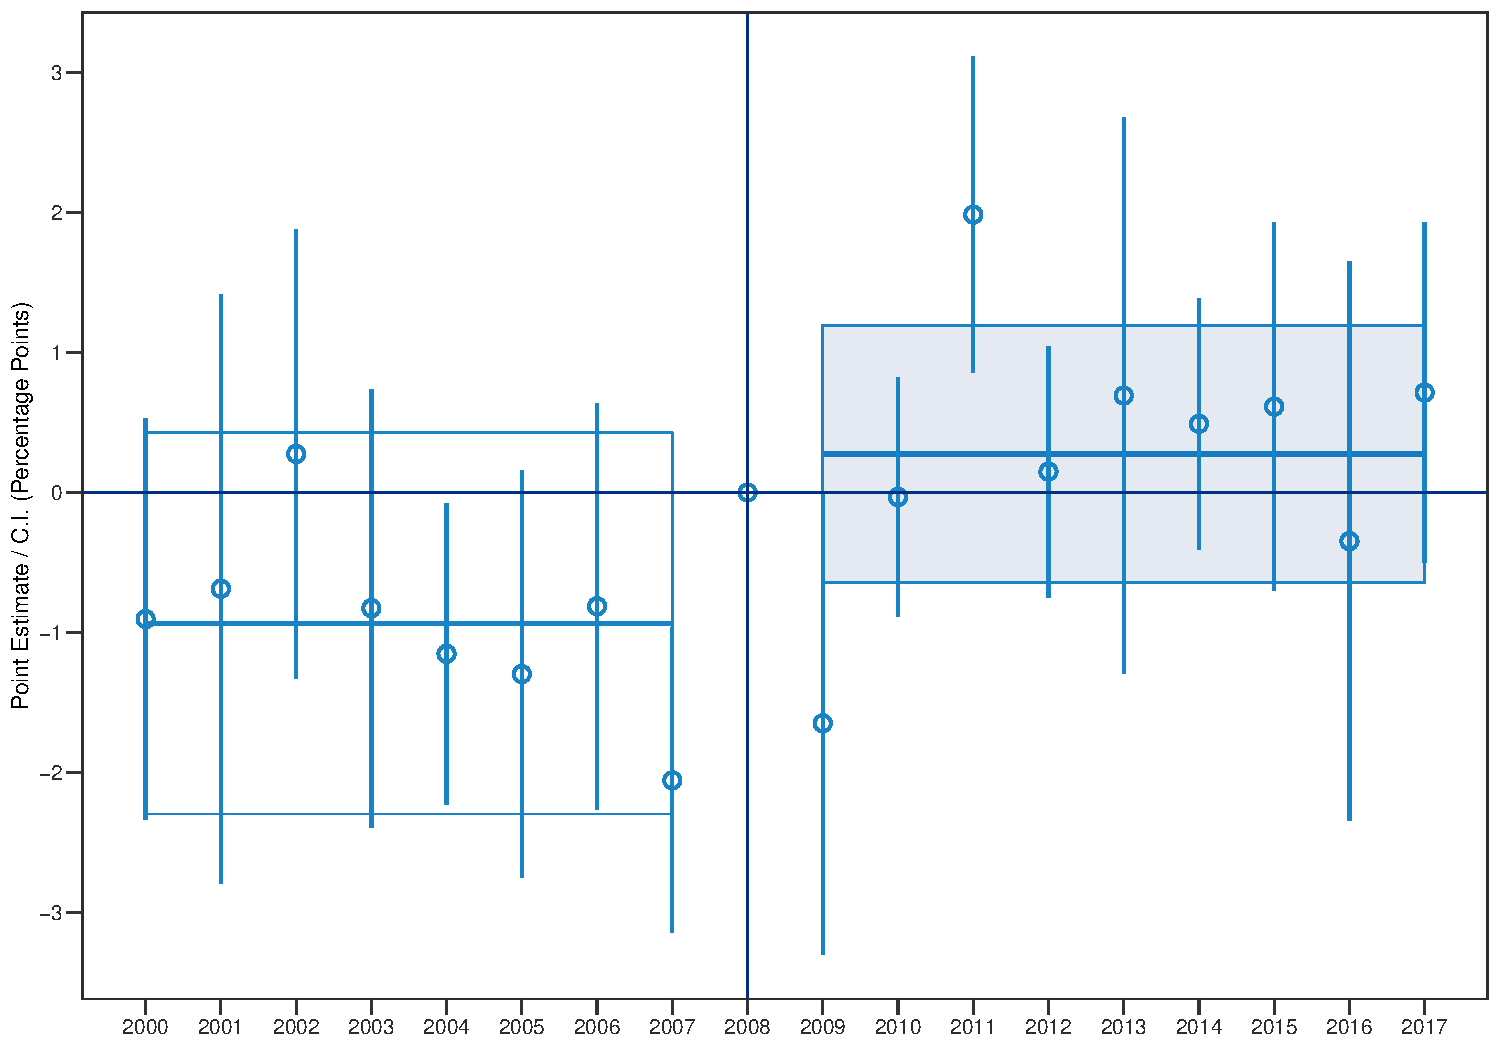
\includegraphics[width=1\linewidth]{events/dynamic_did_cbk_past_mean_pp_p90_noife}
    \begin{tablenotes}
        \footnotesize
        \item \textbf{Notes:}~This table shows ... \hl{XXX}.
    \end{tablenotes} 
\end{figure}

\begin{figure}[htbp!]
    \centering
    \caption{Event Study Plot: Populist Party - Cutoff $90^{th}$ Percentile (with individual FE)}\label{fig:dynamic_did_cbk_past_mean_pp_p90_ife}
    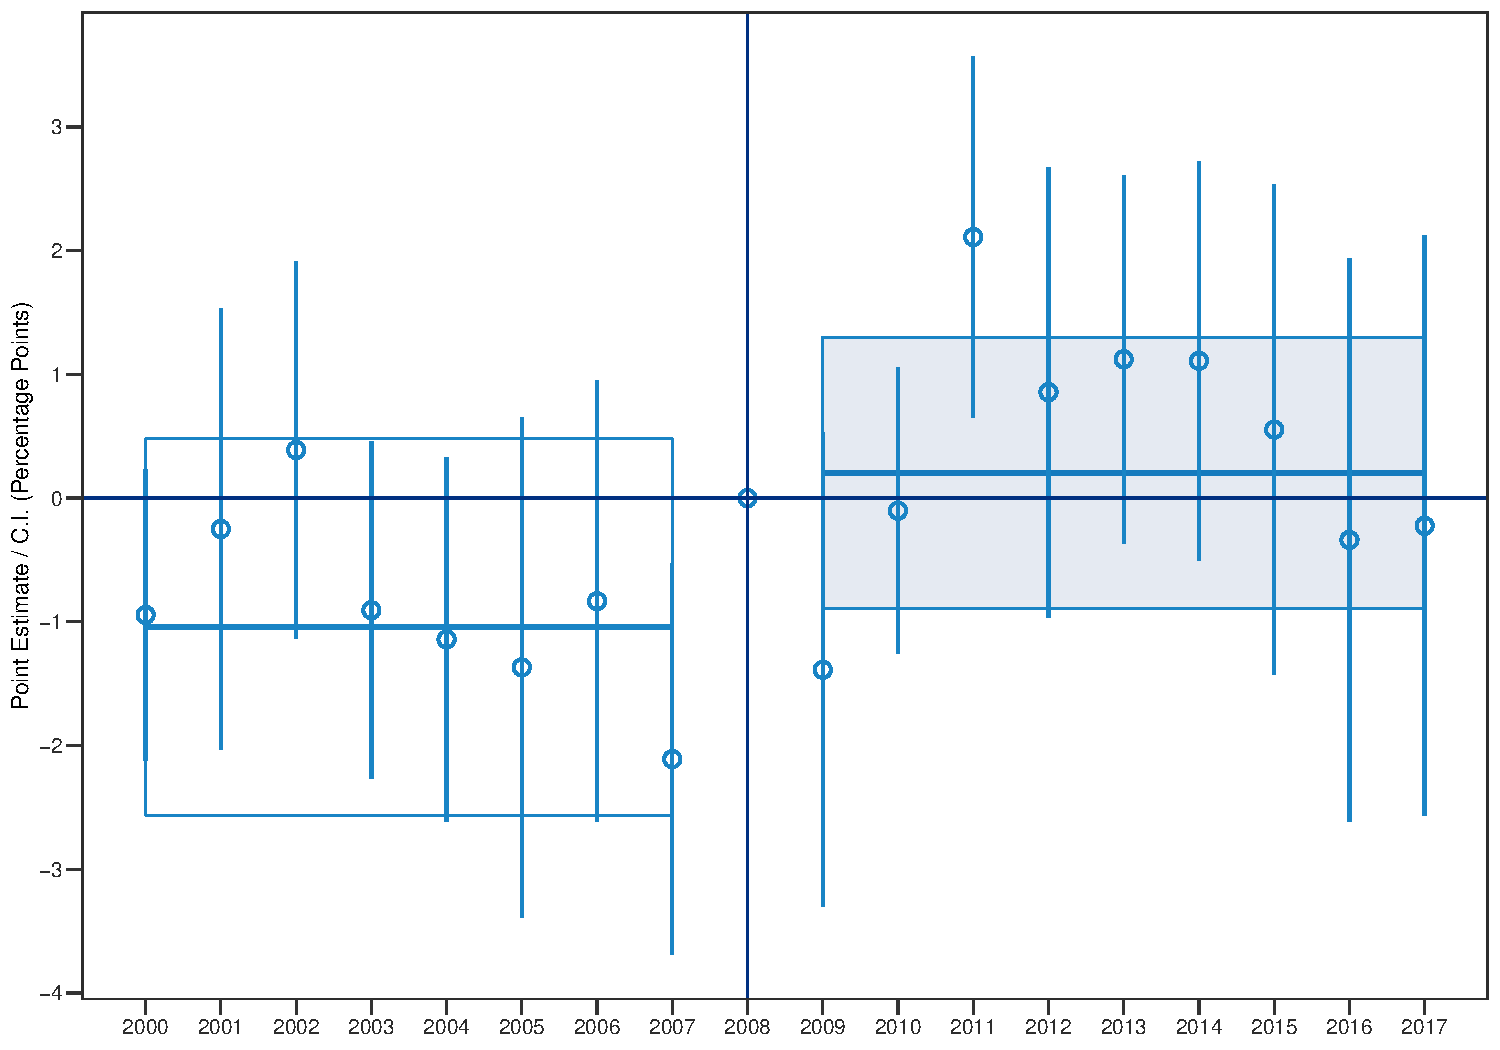
\includegraphics[width=1\linewidth]{events/dynamic_did_cbk_past_mean_pp_p90_ife}
    \begin{tablenotes}
        \footnotesize
        \item \textbf{Notes:}~This table shows ... \hl{XXX}.
    \end{tablenotes} 
\end{figure}

\begin{figure}[htbp!]
    \centering
    \caption{Event Study Plot: Political Support - Cutoff IQR (without individual FE)}\label{fig:dynamic_did_cbk_past_mean_ps_iqr_noife}
    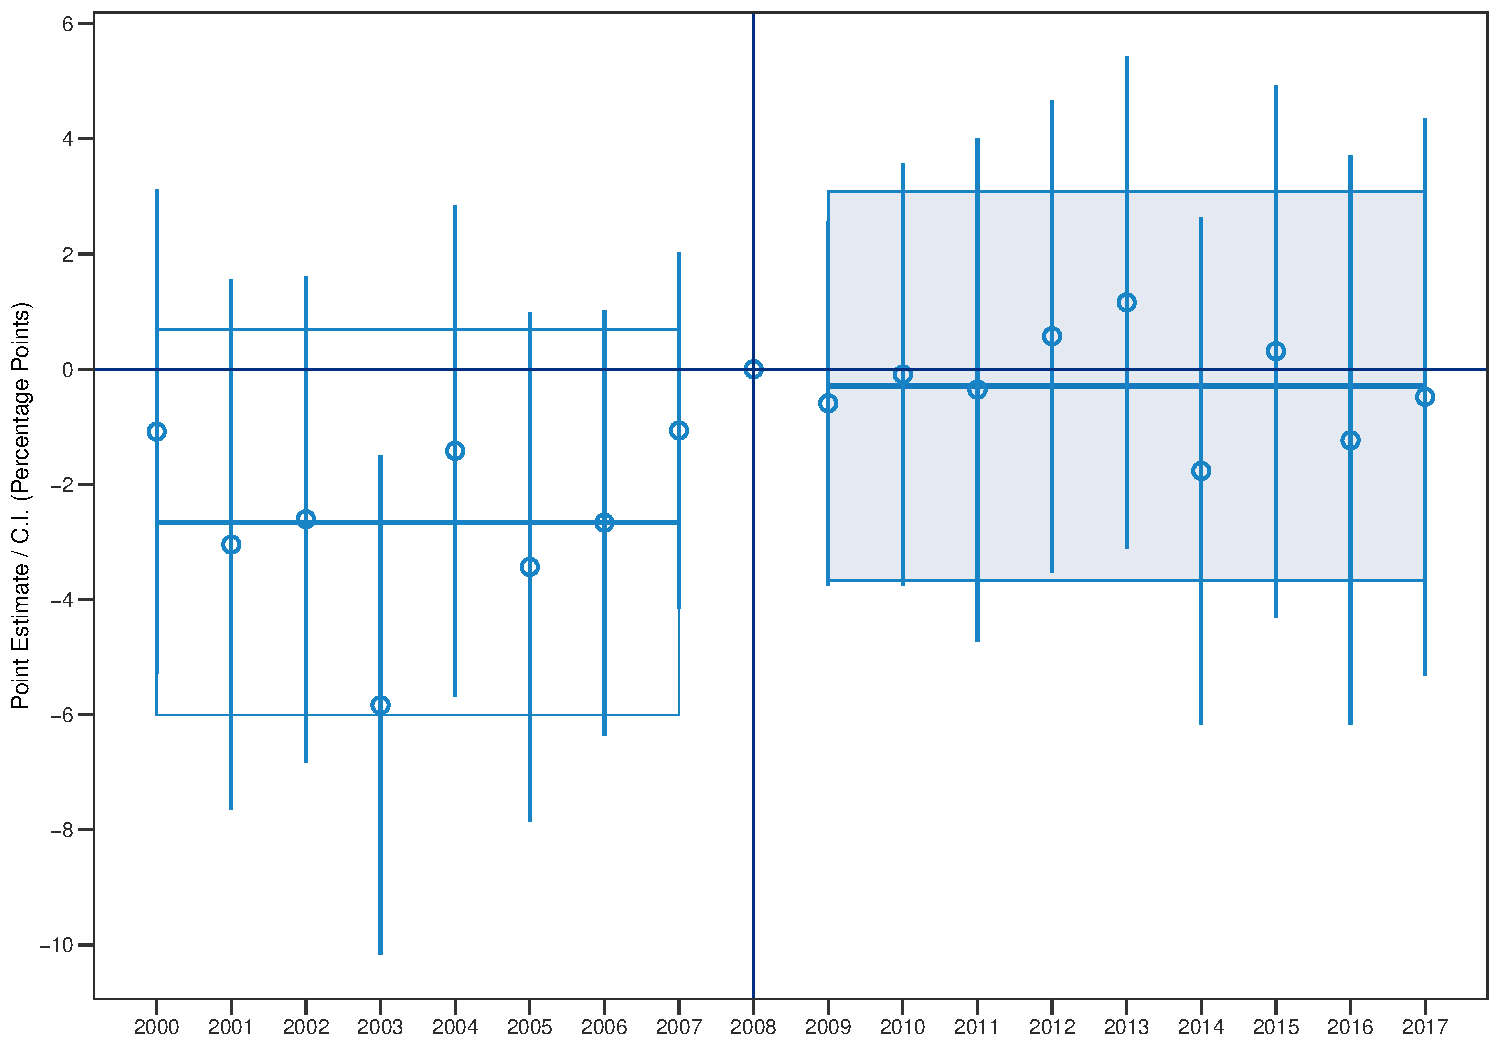
\includegraphics[width=1\linewidth]{events/dynamic_did_cbk_past_mean_ps_iqr_noife}
    \begin{tablenotes}
        \footnotesize
        \item \textbf{Notes:}~This table shows ... \hl{XXX}.
    \end{tablenotes} 
\end{figure}

\begin{figure}[htbp!]
    \centering
    \caption{Event Study Plot: Political Support - Cutoff IQR (with individual FE)}\label{fig:dynamic_did_cbk_past_mean_ps_iqr_ife}
    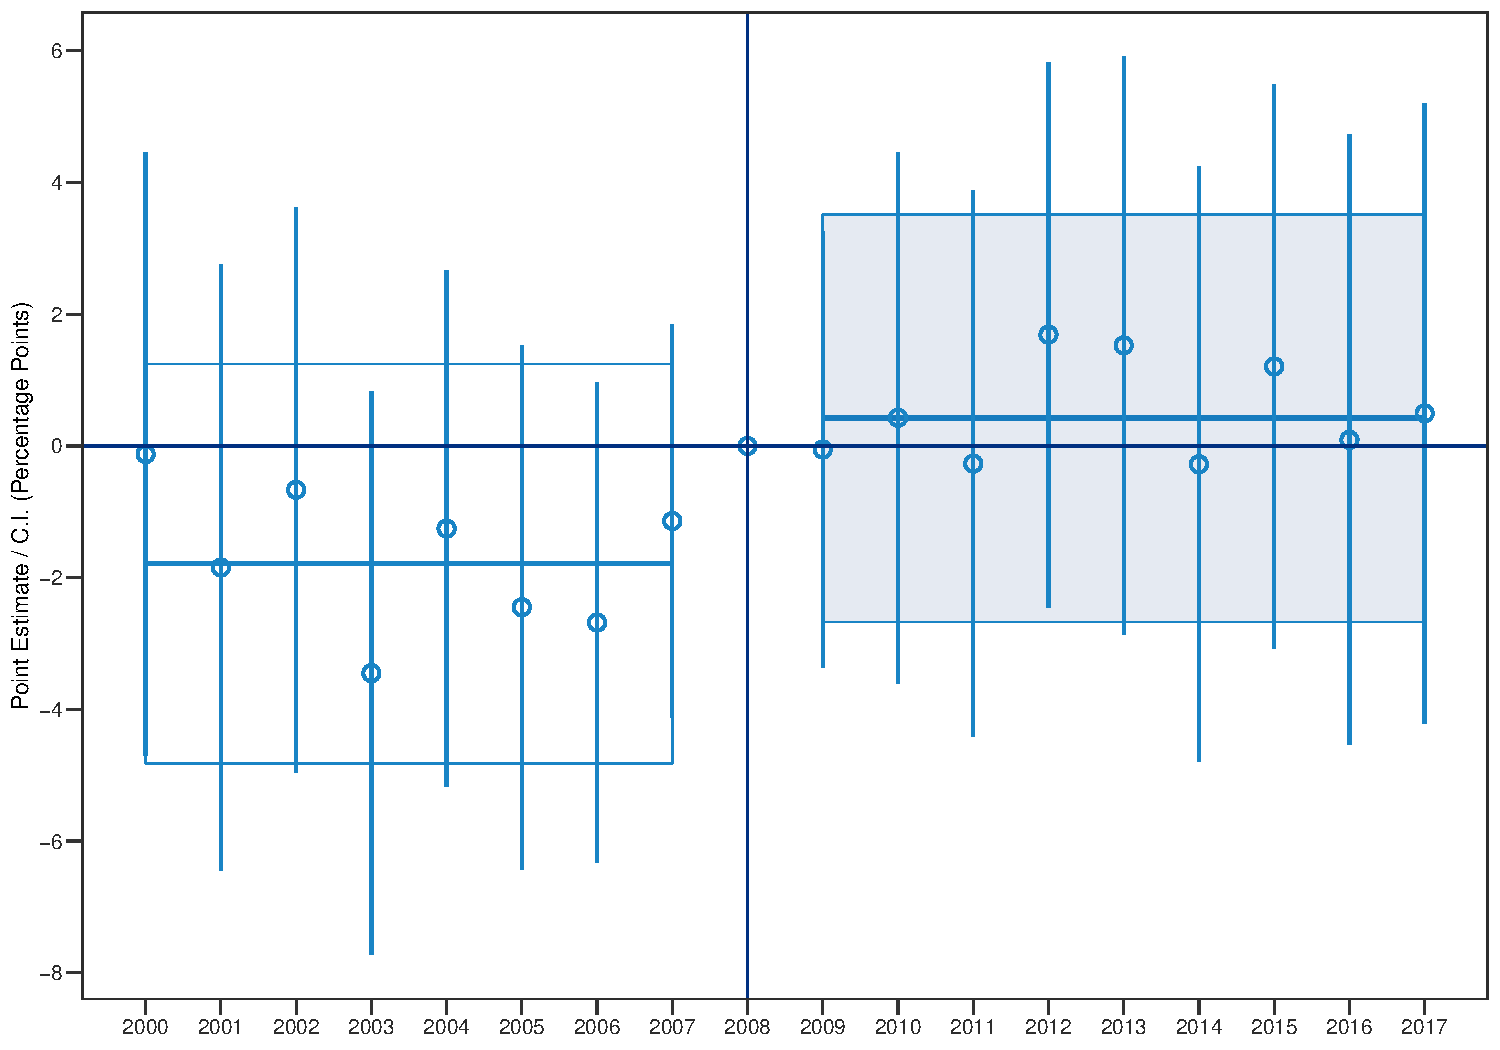
\includegraphics[width=1\linewidth]{events/dynamic_did_cbk_past_mean_ps_iqr_ife}
    \begin{tablenotes}
        \footnotesize
        \item \textbf{Notes:}~This table shows ... \hl{XXX}.
    \end{tablenotes} 
\end{figure}

\begin{figure}[htbp!]
    \centering
    \caption{Event Study Plot: Populist Party - Cutoff IQR (without individual FE)}\label{fig:dynamic_did_cbk_past_mean_pp_iqr_noife}
    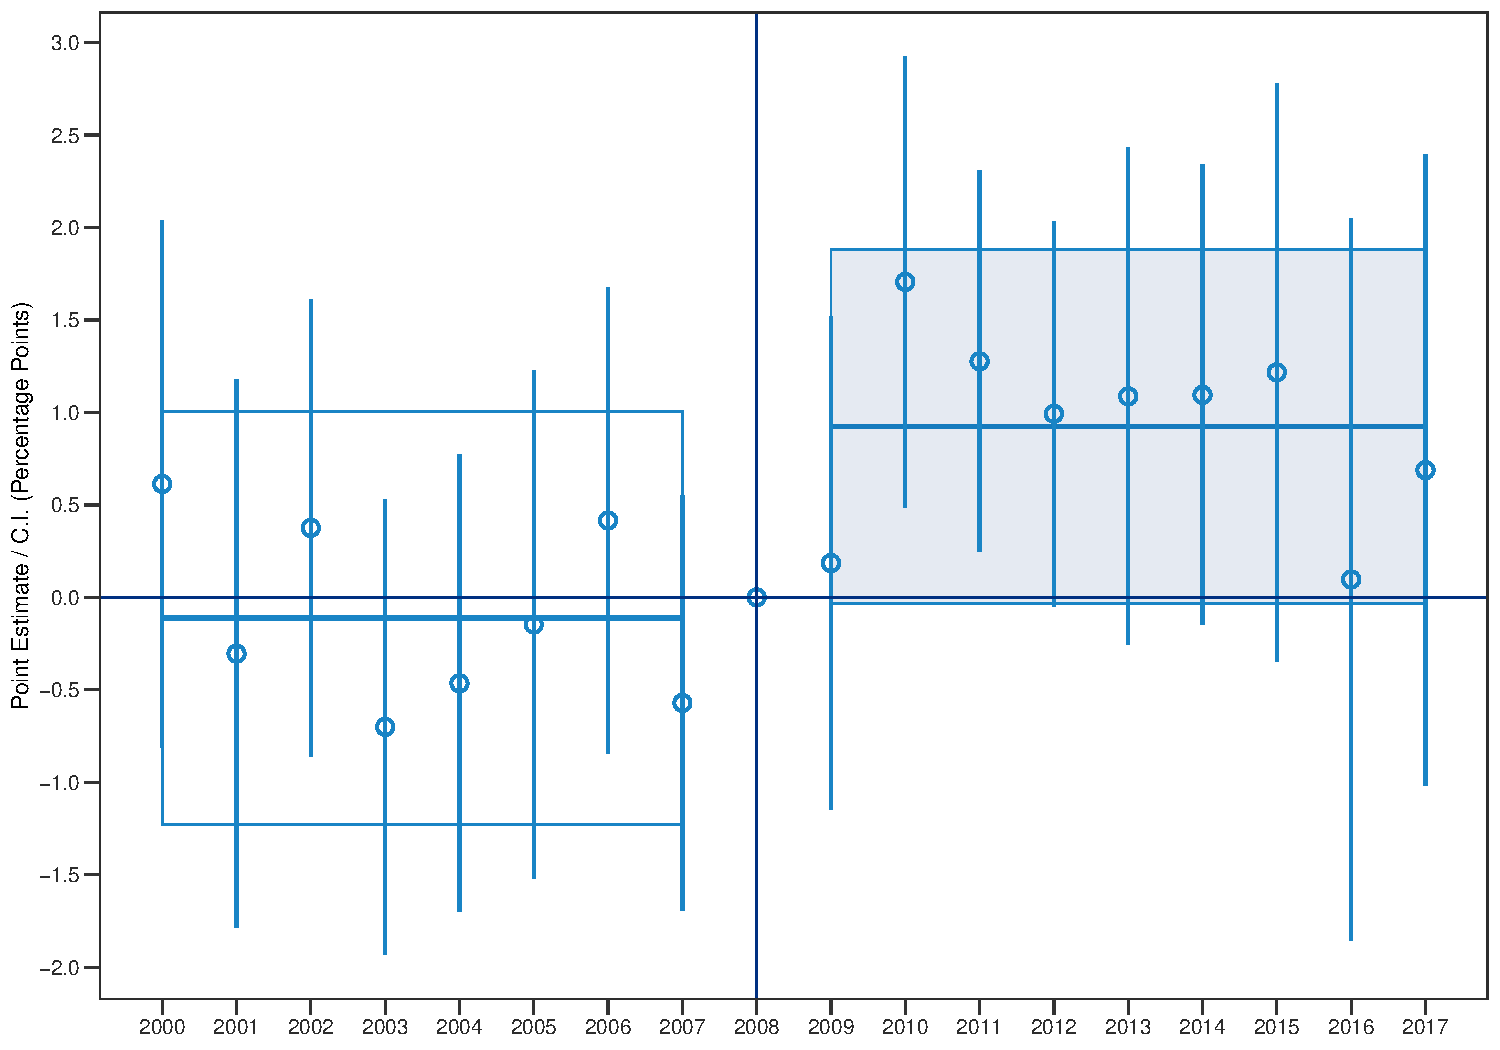
\includegraphics[width=1\linewidth]{events/dynamic_did_cbk_past_mean_pp_iqr_noife}
    \begin{tablenotes}
        \footnotesize
        \item \textbf{Notes:}~This table shows ... \hl{XXX}.
    \end{tablenotes} 
\end{figure}

\begin{figure}[htbp!]
    \centering
    \caption{Event Study Plot: Populist Party - Cutoff IQR (with individual FE)}\label{fig:dynamic_did_cbk_past_mean_pp_iqr_ife}
    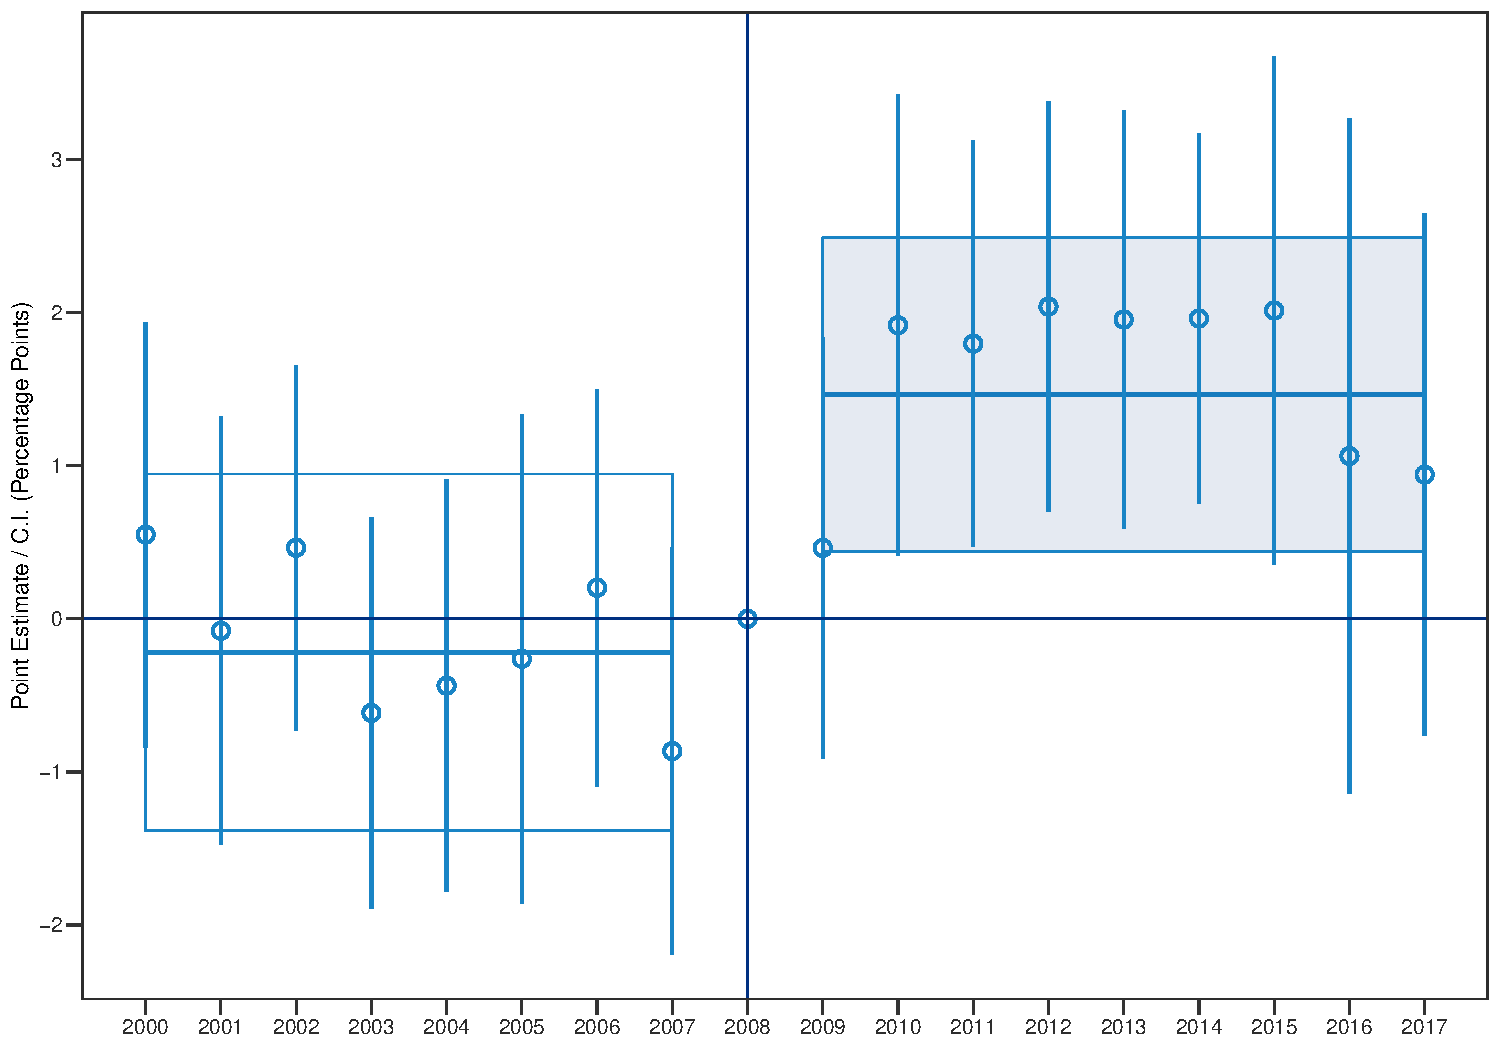
\includegraphics[width=1\linewidth]{events/dynamic_did_cbk_past_mean_pp_iqr_ife}
    \begin{tablenotes}
        \footnotesize
        \item \textbf{Notes:}~This table shows ... \hl{XXX}.
    \end{tablenotes} 
\end{figure}

\begin{figure}[htbp!]
    \centering
    \caption{Event Study Plot: Political Support - Cutoff $10^{th}$--$90^{th}$ Percentile (without individual FE)}\label{fig:dynamic_did_cbk_past_mean_ps_1090_noife}
    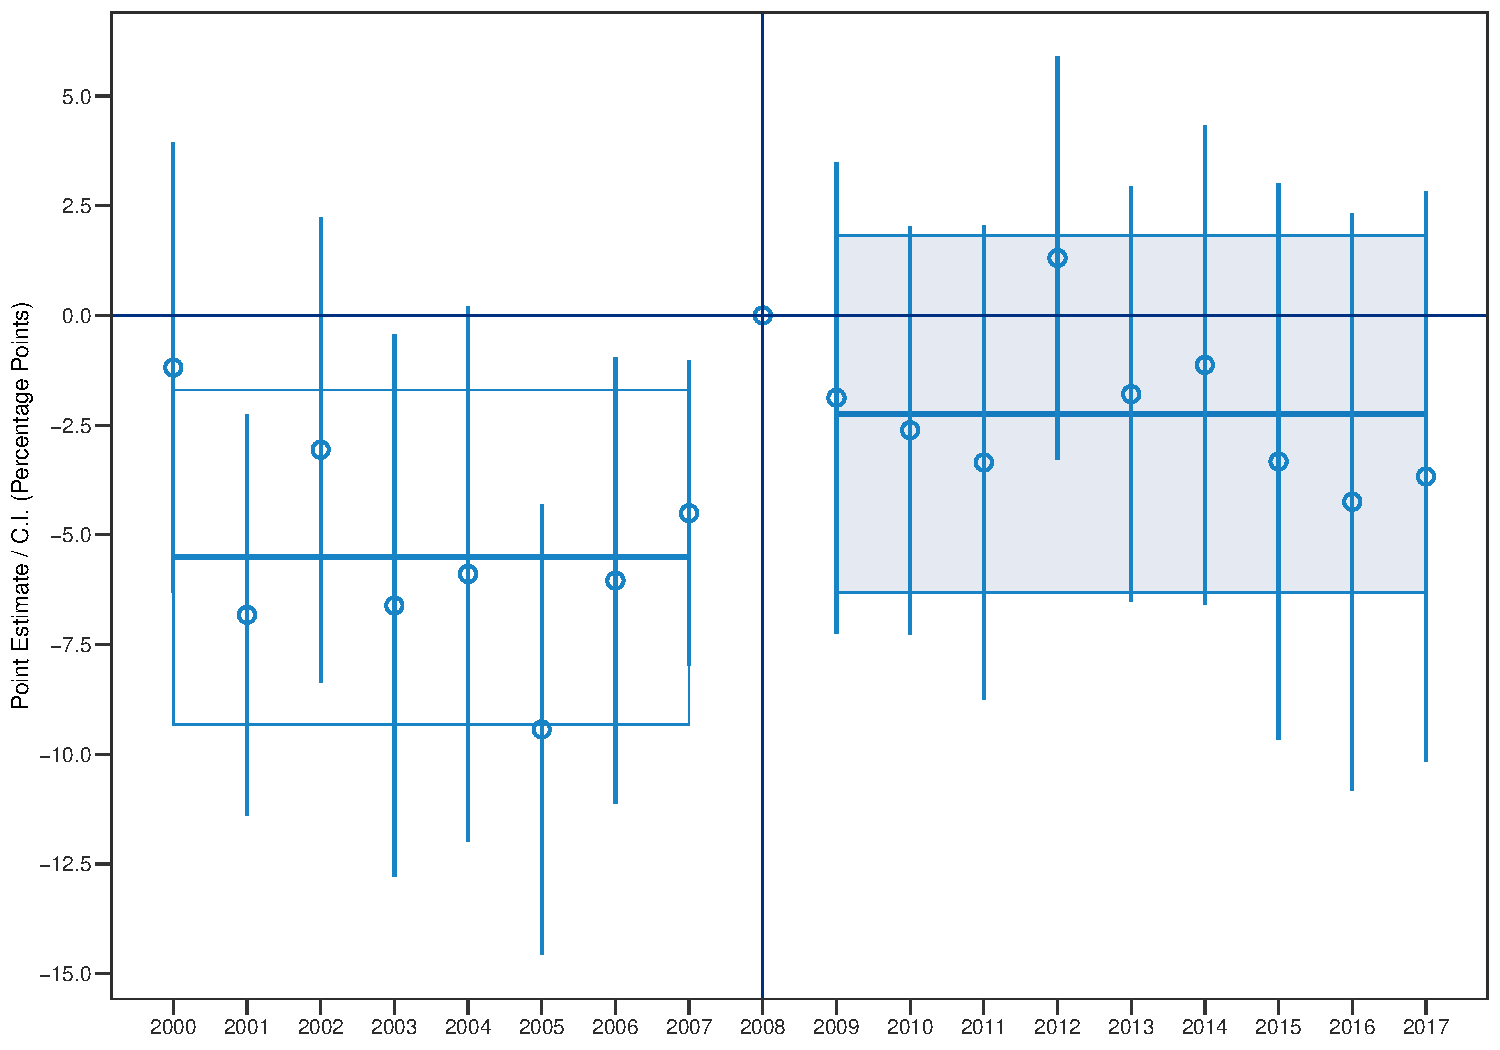
\includegraphics[width=1\linewidth]{events/dynamic_did_cbk_past_mean_ps_1090_noife}
    \begin{tablenotes}
        \footnotesize
        \item \textbf{Notes:}~This table shows ... \hl{XXX}.
    \end{tablenotes} 
\end{figure}

\begin{figure}[htbp!]
    \centering
    \caption{Event Study Plot: Political Support - Cutoff $10^{th}$--$90^{th}$ Percentile (with individual FE)}\label{fig:dynamic_did_cbk_past_mean_ps_1090_ife}
    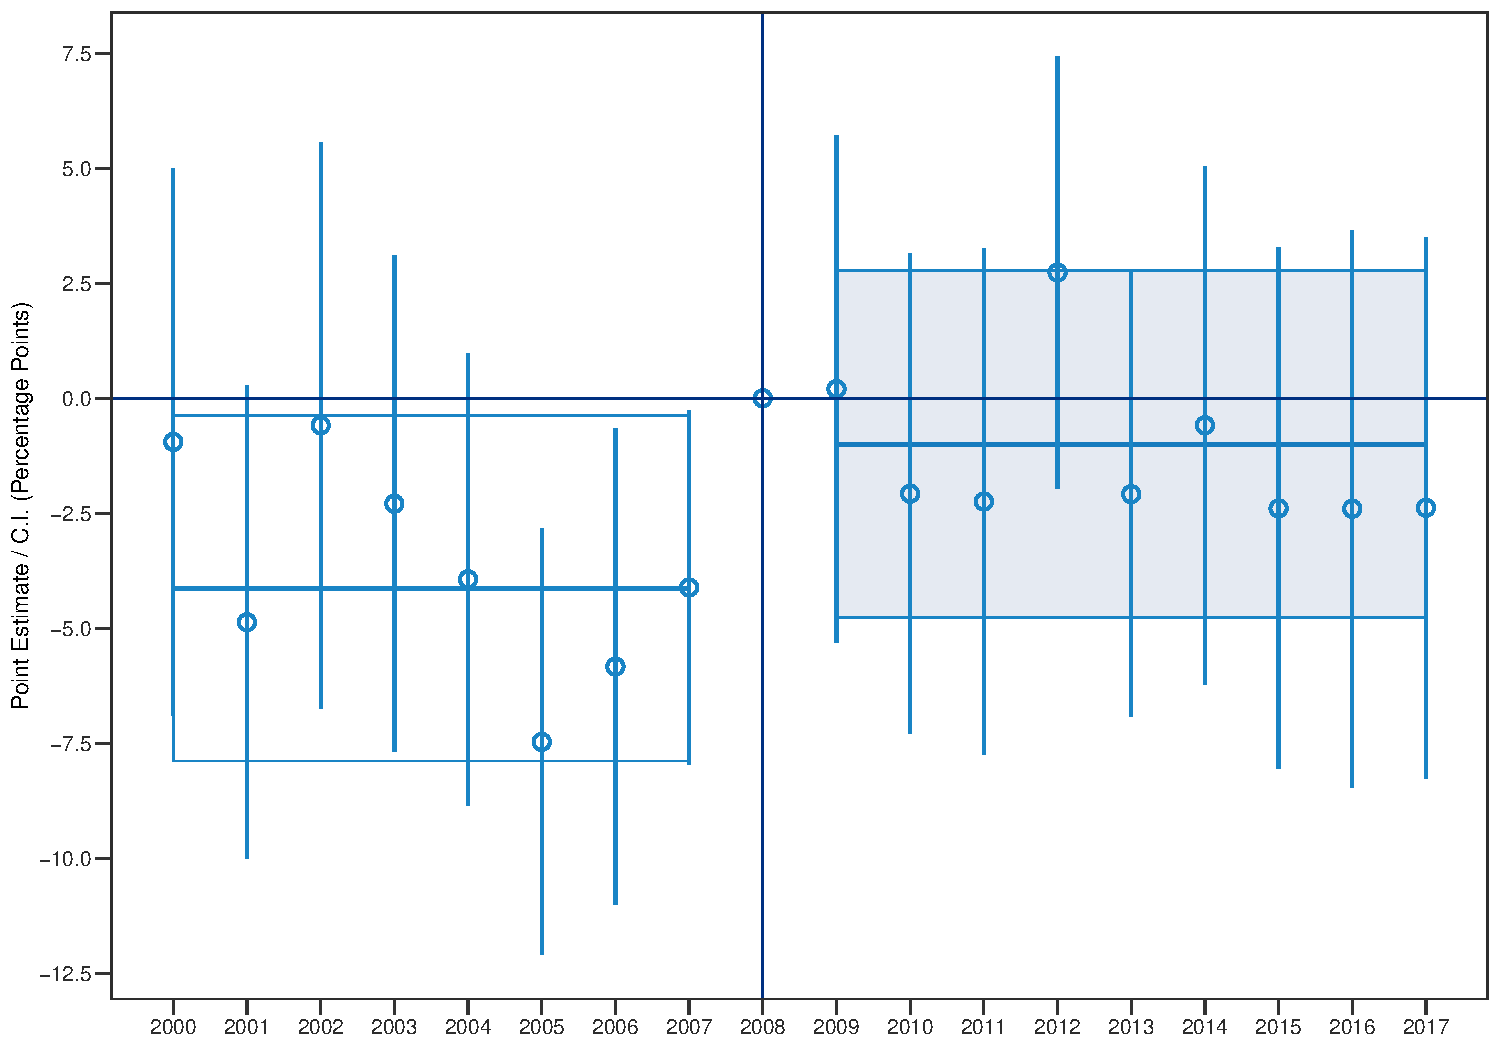
\includegraphics[width=1\linewidth]{events/dynamic_did_cbk_past_mean_ps_1090_ife}
    \begin{tablenotes}
        \footnotesize
        \item \textbf{Notes:}~This table shows ... \hl{XXX}.
    \end{tablenotes} 
\end{figure}

\begin{figure}[htbp!]
    \centering
    \caption{Event Study Plot: Populist Party - Cutoff $10^{th}$--$90^{th}$ Percentile (without individual FE)}\label{fig:dynamic_did_cbk_past_mean_pp_1090_noife}
    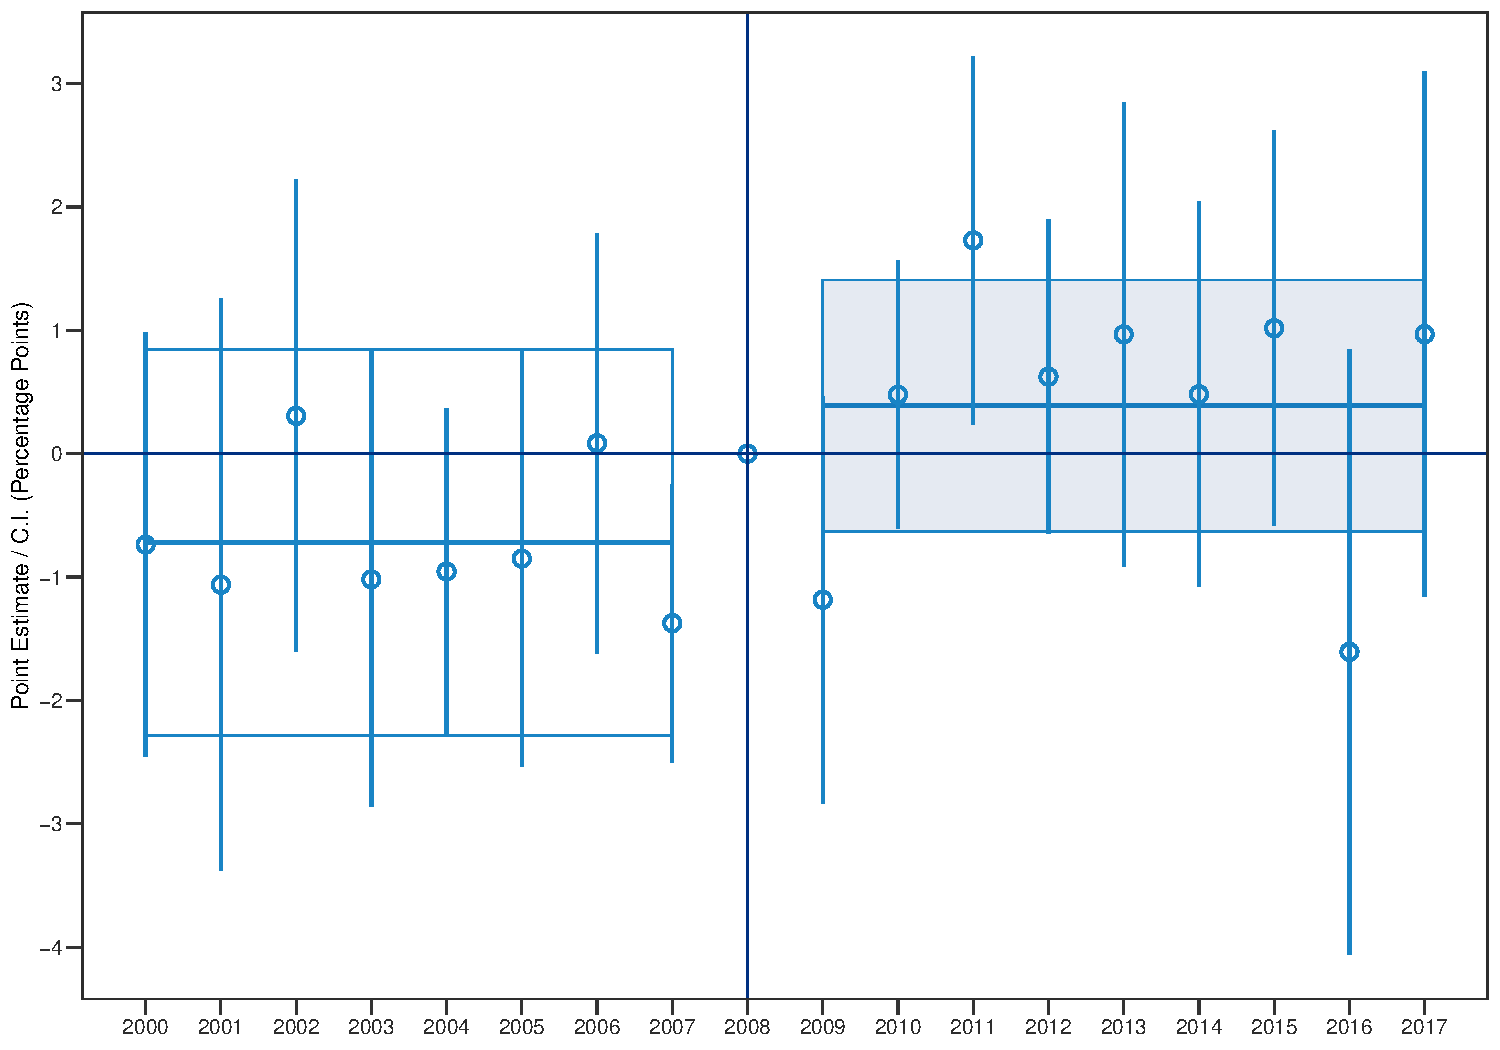
\includegraphics[width=1\linewidth]{events/dynamic_did_cbk_past_mean_pp_1090_noife}
    \begin{tablenotes}
        \footnotesize
        \item \textbf{Notes:}~This table shows ... \hl{XXX}.
    \end{tablenotes} 
\end{figure}

\begin{figure}[htbp!]
    \centering
    \caption{Event Study Plot: Populist Party - Cutoff $10^{th}$--$90^{th}$ Percentile (with individual FE)}\label{fig:dynamic_did_cbk_past_mean_pp_1090_ife}
    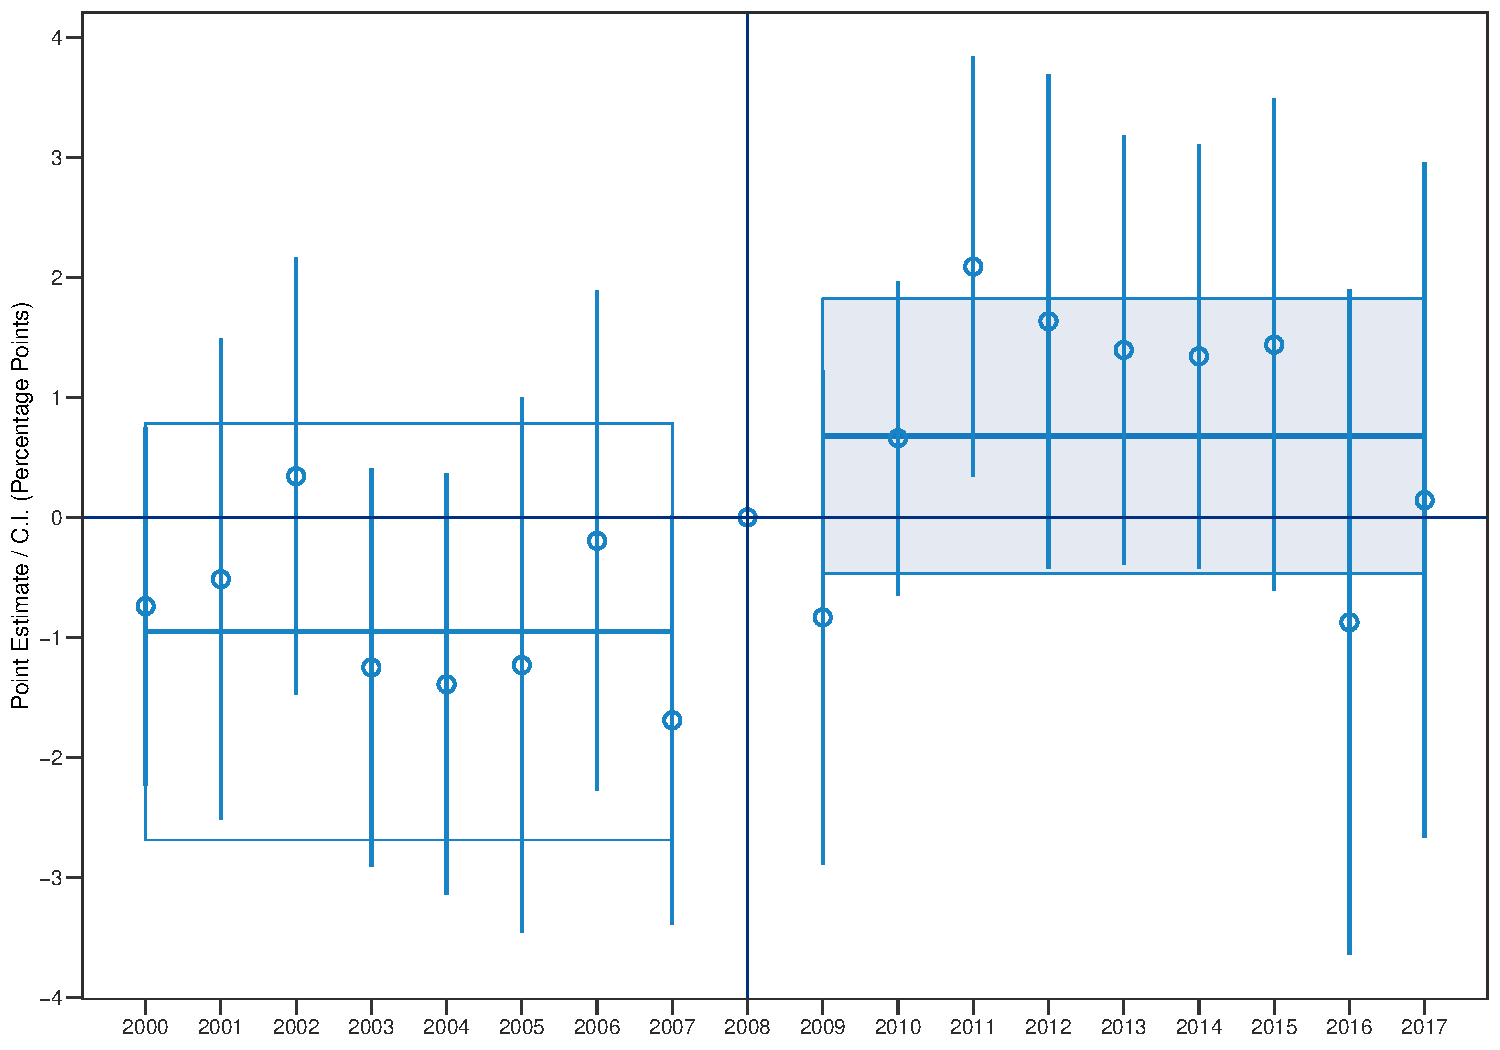
\includegraphics[width=1\linewidth]{events/dynamic_did_cbk_past_mean_pp_1090_ife}
    \begin{tablenotes}
        \footnotesize
        \item \textbf{Notes:}~This table shows ... \hl{XXX}.
    \end{tablenotes} 
\end{figure}

\begin{figure}[htbp!]
    \centering
    \caption{Event Study Plot: Political Support - Continuous Treatment (without individual FE)}\label{fig:dynamic_did_cbk_past_mean_ps_std_noife}
    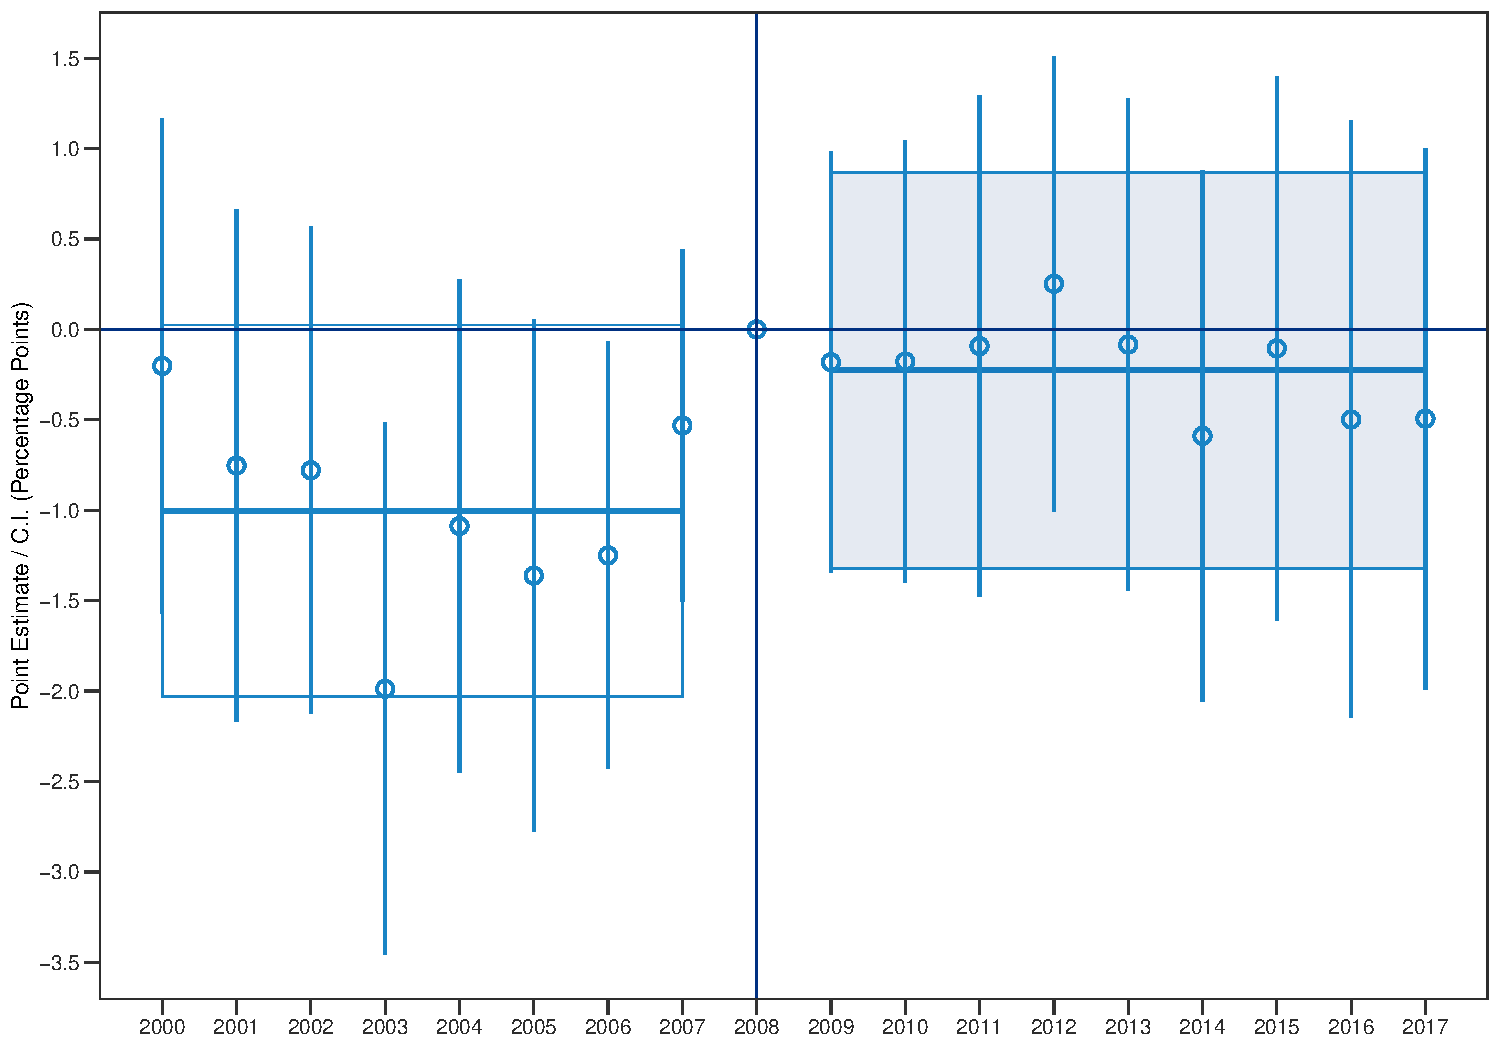
\includegraphics[width=1\linewidth]{events/dynamic_did_cbk_past_mean_ps_std_noife}
    \begin{tablenotes}
        \footnotesize
        \item \textbf{Notes:}~This table shows ... \hl{XXX}.
    \end{tablenotes} 
\end{figure}

\begin{figure}[htbp!]
    \centering
    \caption{Event Study Plot: Political Support - Continuous Treatment (with individual FE)}\label{fig:dynamic_did_cbk_past_mean_ps_std_ife}
    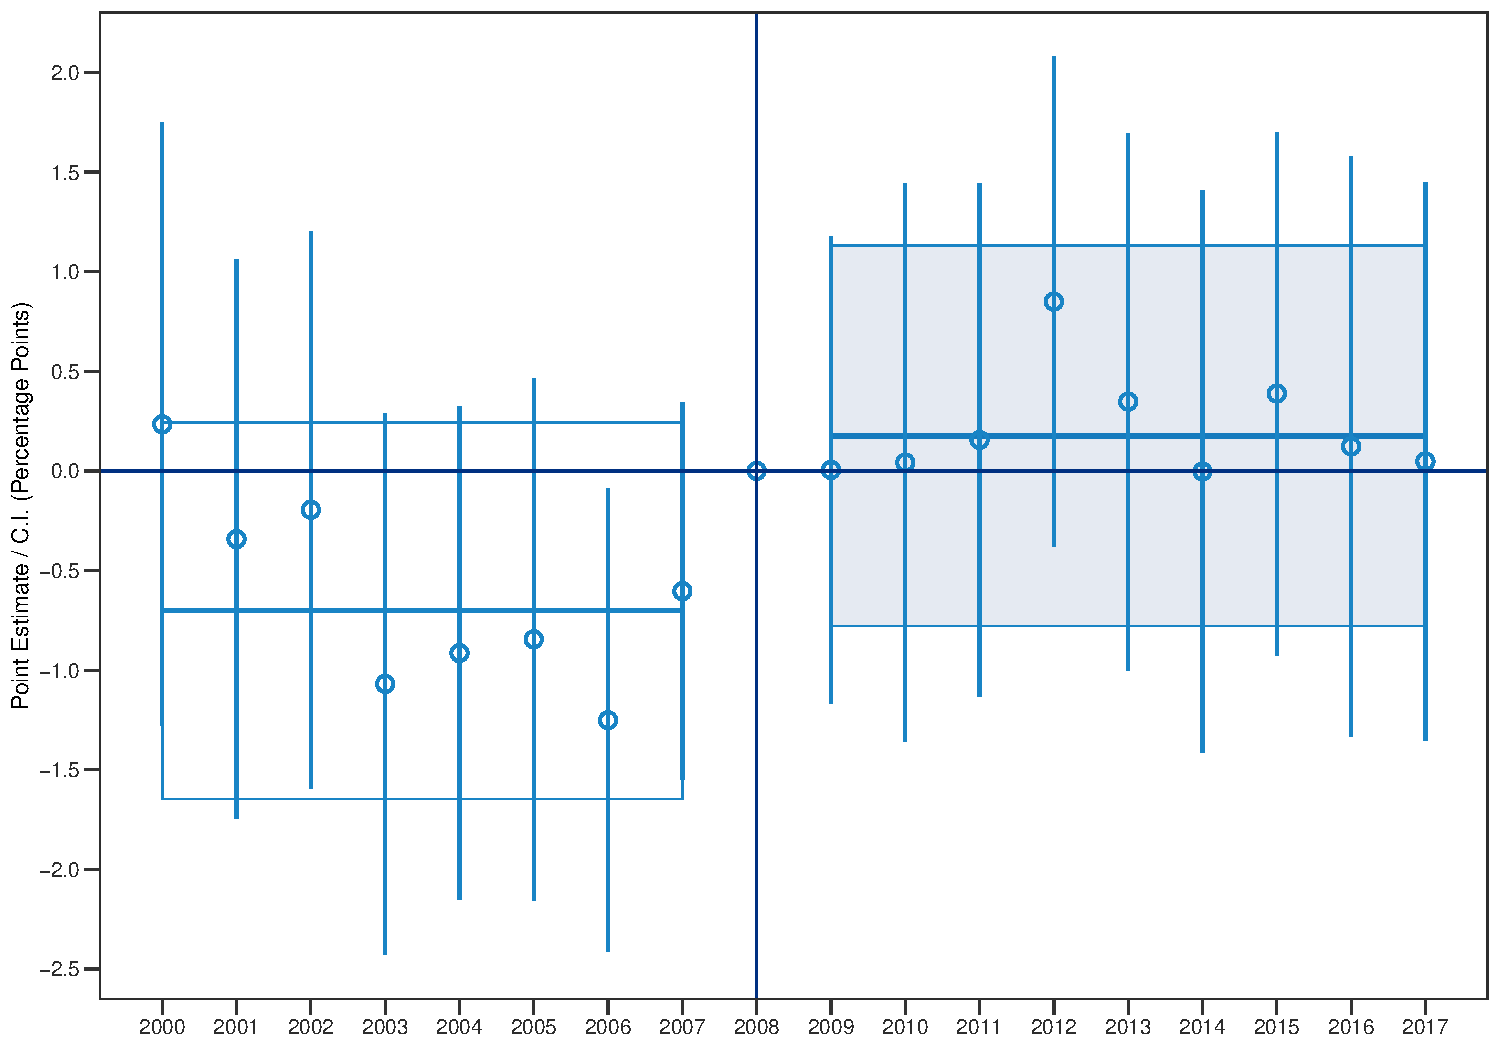
\includegraphics[width=1\linewidth]{events/dynamic_did_cbk_past_mean_ps_std_ife}
    \begin{tablenotes}
        \footnotesize
        \item \textbf{Notes:}~This table shows ... \hl{XXX}.
    \end{tablenotes} 
\end{figure}

\begin{figure}[htbp!]
    \centering
    \caption{Event Study Plot: Populist Party - Continuous Treatment (without individual FE)}\label{fig:dynamic_did_cbk_past_mean_pp_std_noife}
    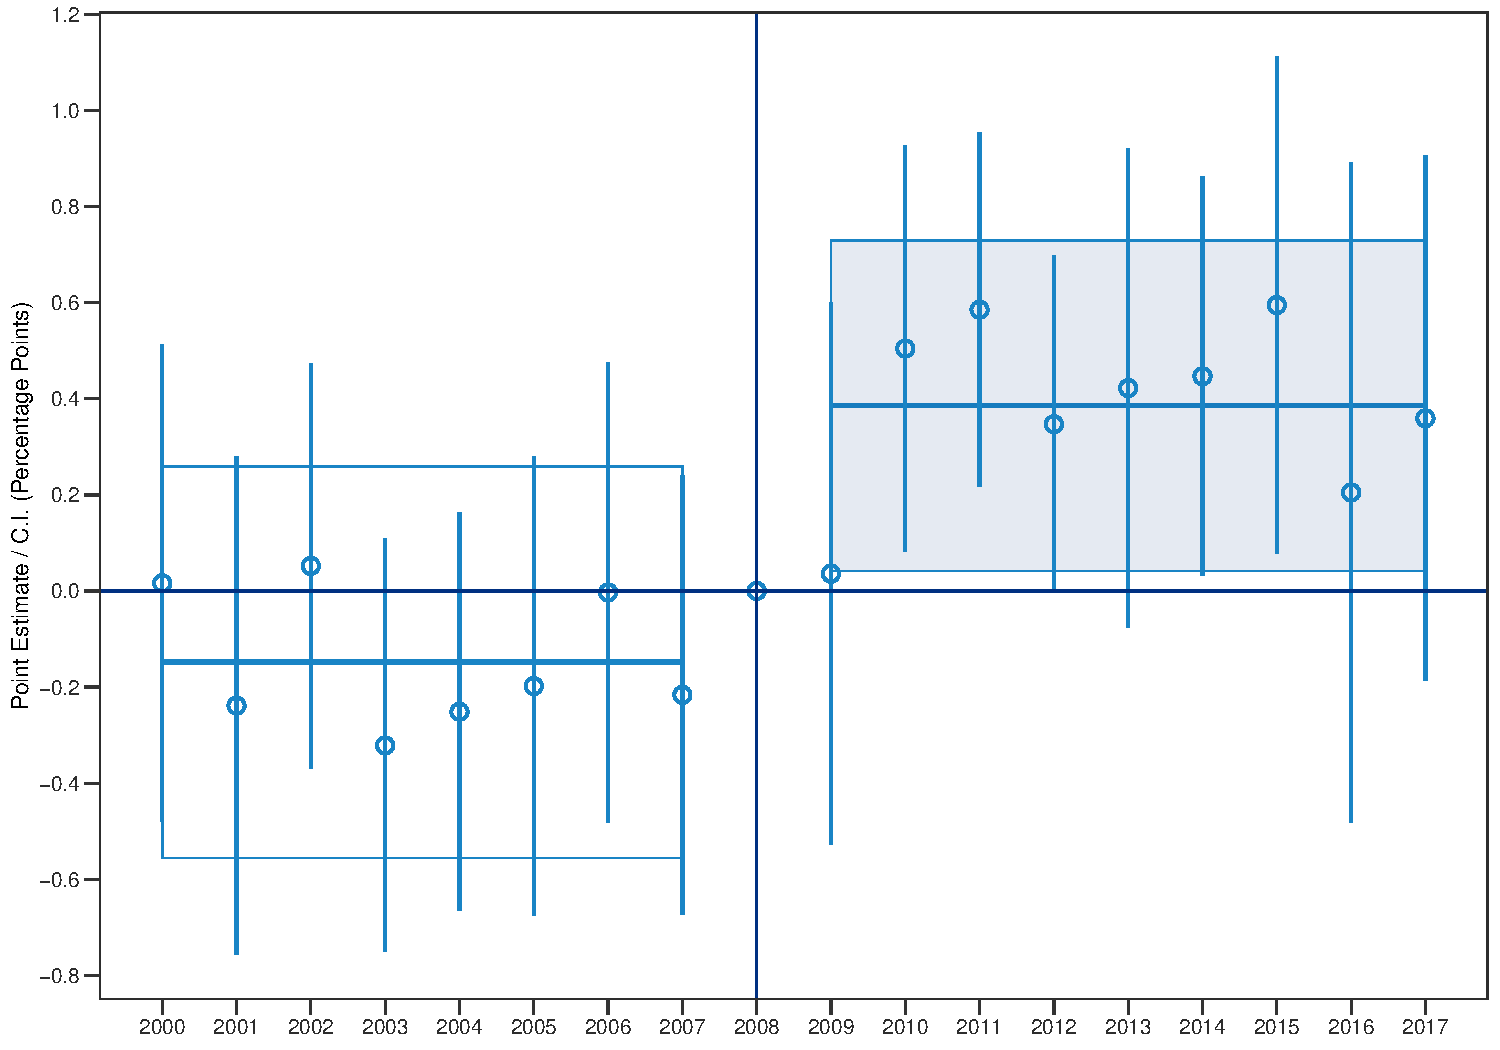
\includegraphics[width=1\linewidth]{events/dynamic_did_cbk_past_mean_pp_std_noife}
    \begin{tablenotes}
        \footnotesize
        \item \textbf{Notes:}~This table shows ... \hl{XXX}.
    \end{tablenotes} 
\end{figure}

\begin{figure}[htbp!]
    \centering
    \caption{Event Study Plot: Populist Party - Continuous Treatment (with individual FE)}\label{fig:dynamic_did_cbk_past_mean_pp_std_ife}
    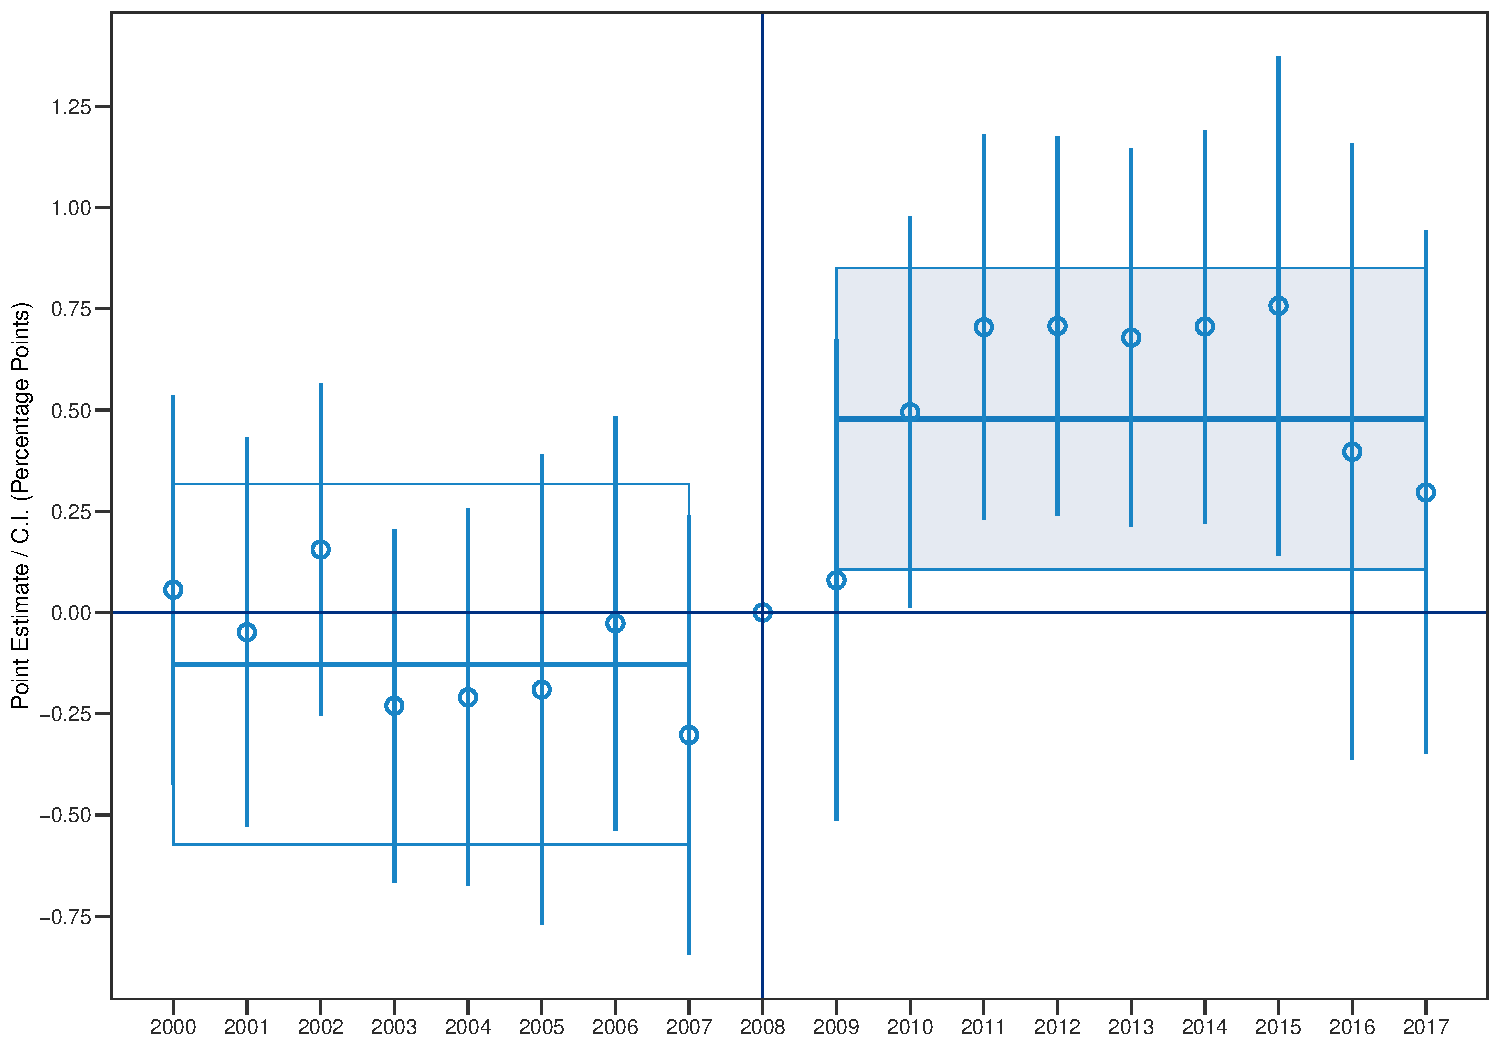
\includegraphics[width=1\linewidth]{events/dynamic_did_cbk_past_mean_pp_std_ife}
    \begin{tablenotes}
        \footnotesize
        \item \textbf{Notes:}~This table shows ... \hl{XXX}.
    \end{tablenotes} 
\end{figure}

%%%%%% FUNCTIONAL FORM FIGURES

\begin{figure}[htbp!]
    \centering
    \caption{Heterogeneity on Political Support: Continuous Treatment Functional Form (without individual FE) Level-Level}\label{fig:ps_functional_form_cbk_past_mean_noife_levels}
    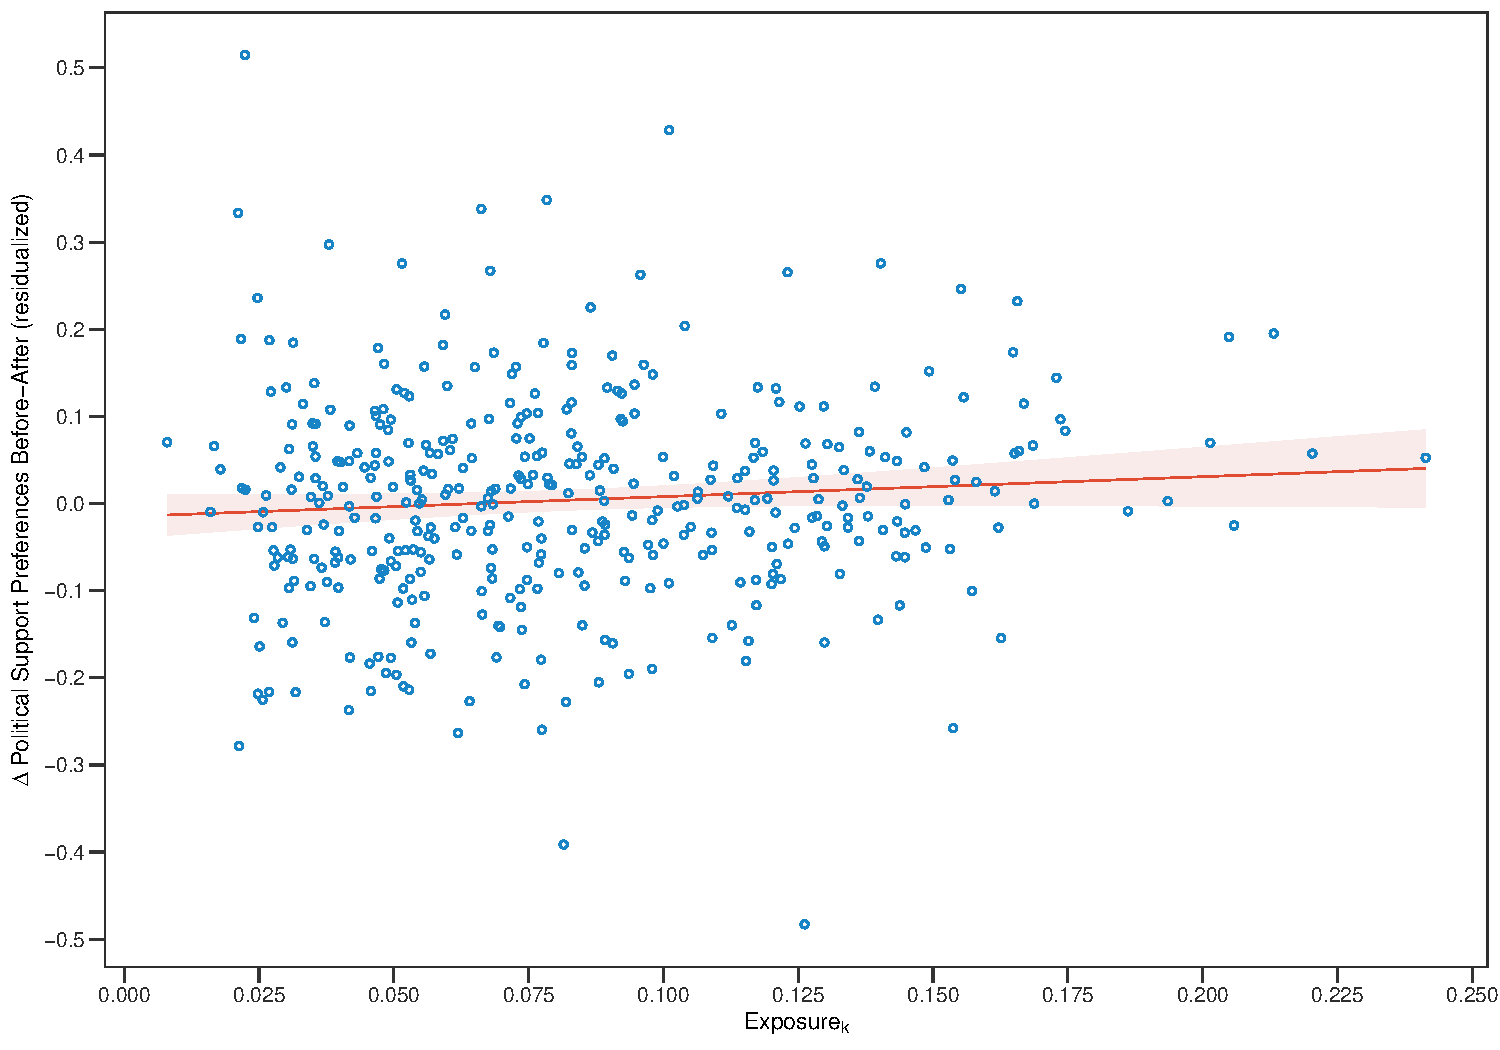
\includegraphics[width=1\linewidth]{heterogeneity/ps_functional_form_cbk_past_mean_noife_levels}
    \begin{tablenotes}
        \footnotesize
        \item \textbf{Notes:}~This table shows ... \hl{XXX}.
    \end{tablenotes} 
\end{figure}

\begin{figure}[htbp!]
    \centering
    \caption{Heterogeneity on Political Support: Continuous Treatment Functional Form (with individual FE) Level-Level}\label{fig:ps_functional_form_cbk_past_mean_ife_levels}
    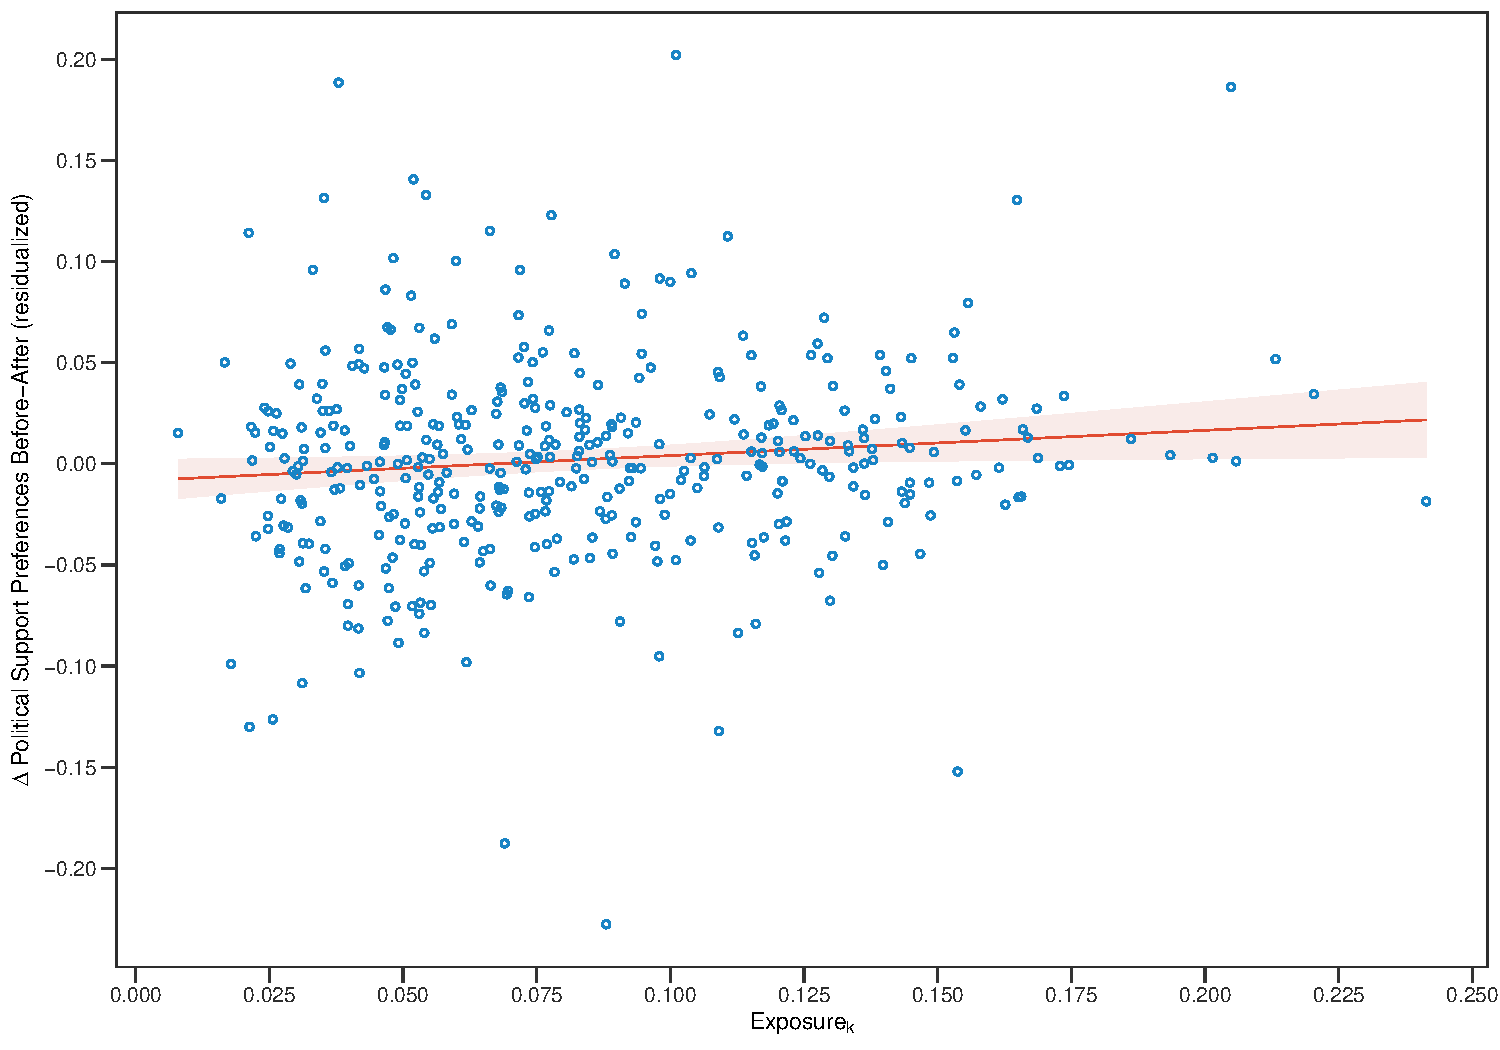
\includegraphics[width=1\linewidth]{heterogeneity/ps_functional_form_cbk_past_mean_ife_levels}
    \begin{tablenotes}
        \footnotesize
        \item \textbf{Notes:}~This table shows ... \hl{XXX}.
    \end{tablenotes} 
\end{figure}

\begin{figure}[htbp!]
    \centering
    \caption{Heterogeneity on Populist Party: Continuous Treatment Functional Form (without individual FE) Level-Level}\label{fig:pp_functional_form_cbk_past_mean_noife_levels}
    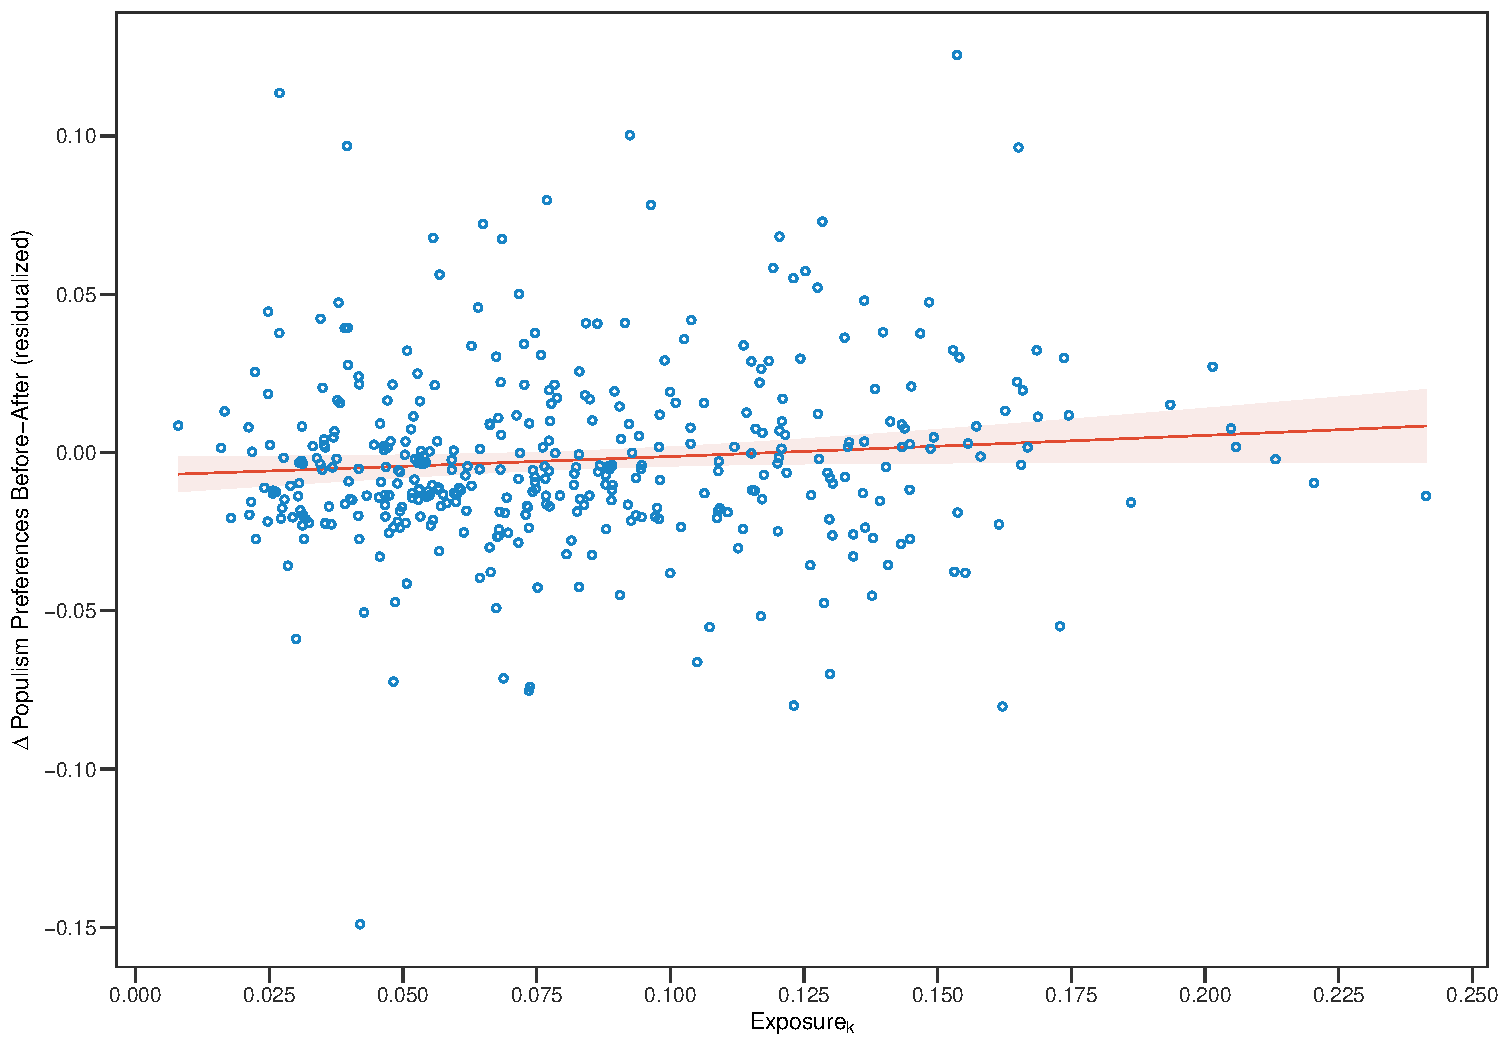
\includegraphics[width=1\linewidth]{heterogeneity/pp_functional_form_cbk_past_mean_noife_levels}
    \begin{tablenotes}
        \footnotesize
        \item \textbf{Notes:}~This table shows ... \hl{XXX}.
    \end{tablenotes} 
\end{figure}

\begin{figure}[htbp!]
    \centering
    \caption{Heterogeneity on Populist Party: Continuous Treatment Functional Form (with individual FE) Level-Level}\label{fig:pp_functional_form_cbk_past_mean_ife_levels}
    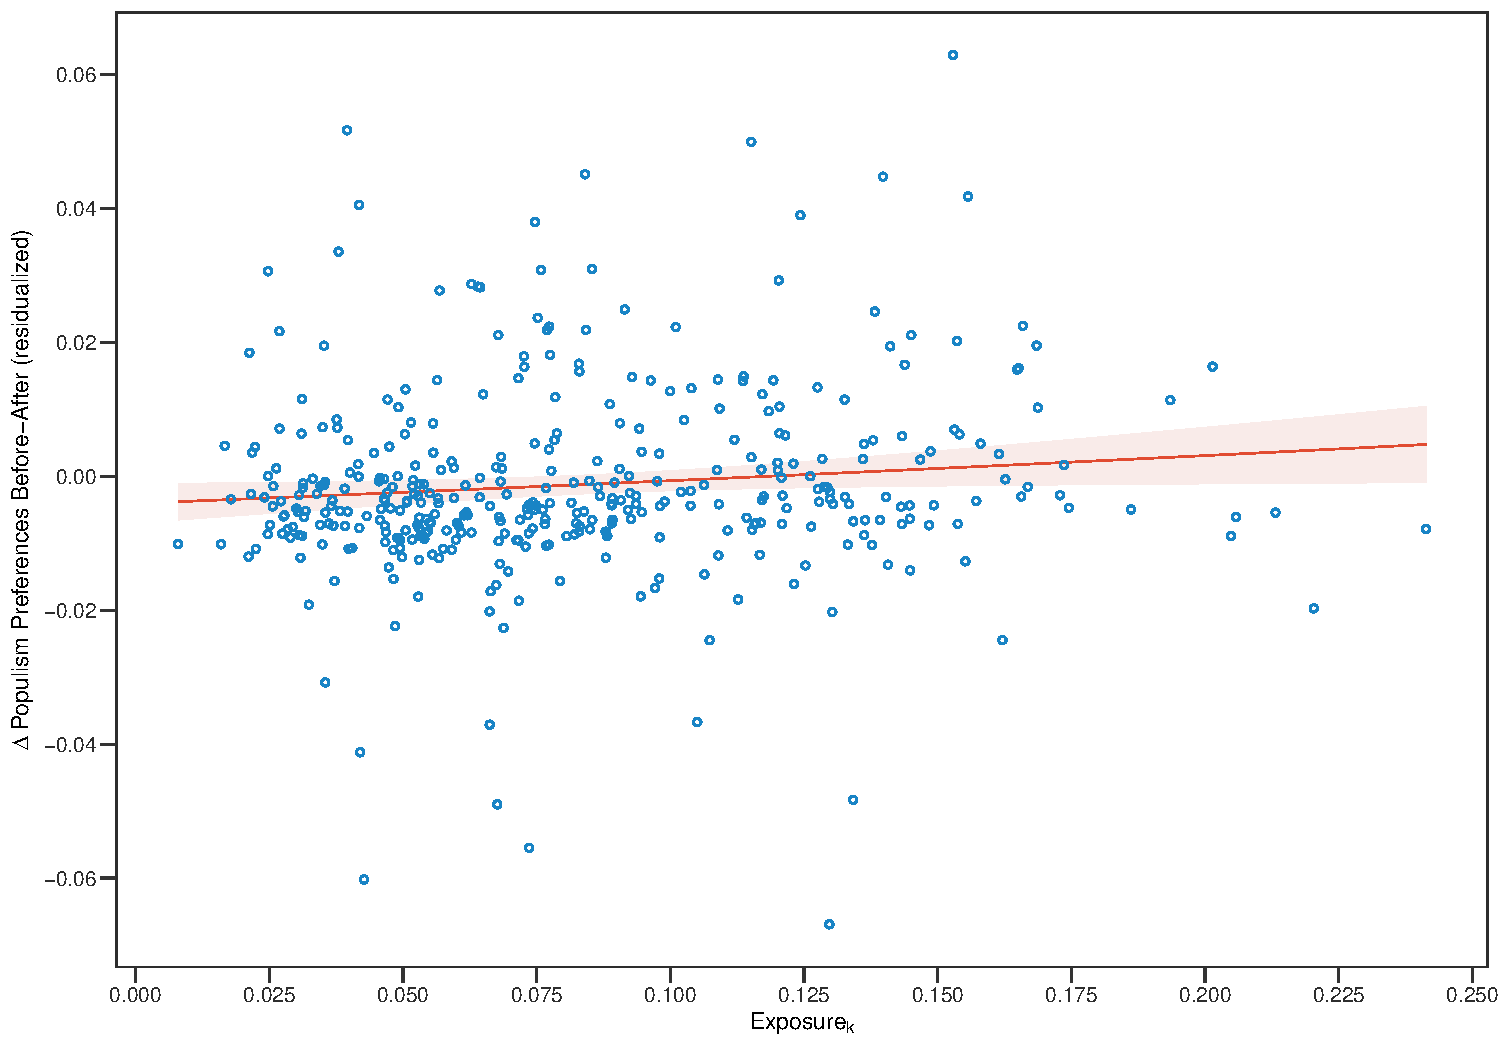
\includegraphics[width=1\linewidth]{heterogeneity/pp_functional_form_cbk_past_mean_ife_levels}
    \begin{tablenotes}
        \footnotesize
        \item \textbf{Notes:}~This table shows ... \hl{XXX}.
    \end{tablenotes} 
\end{figure}

\begin{figure}[htbp!]
    \centering
    \caption{Heterogeneity on Political Support: Continuous Treatment Functional Form (without individual FE) Log-Log}\label{fig:ps_functional_form_cbk_past_mean_noife_logs}
    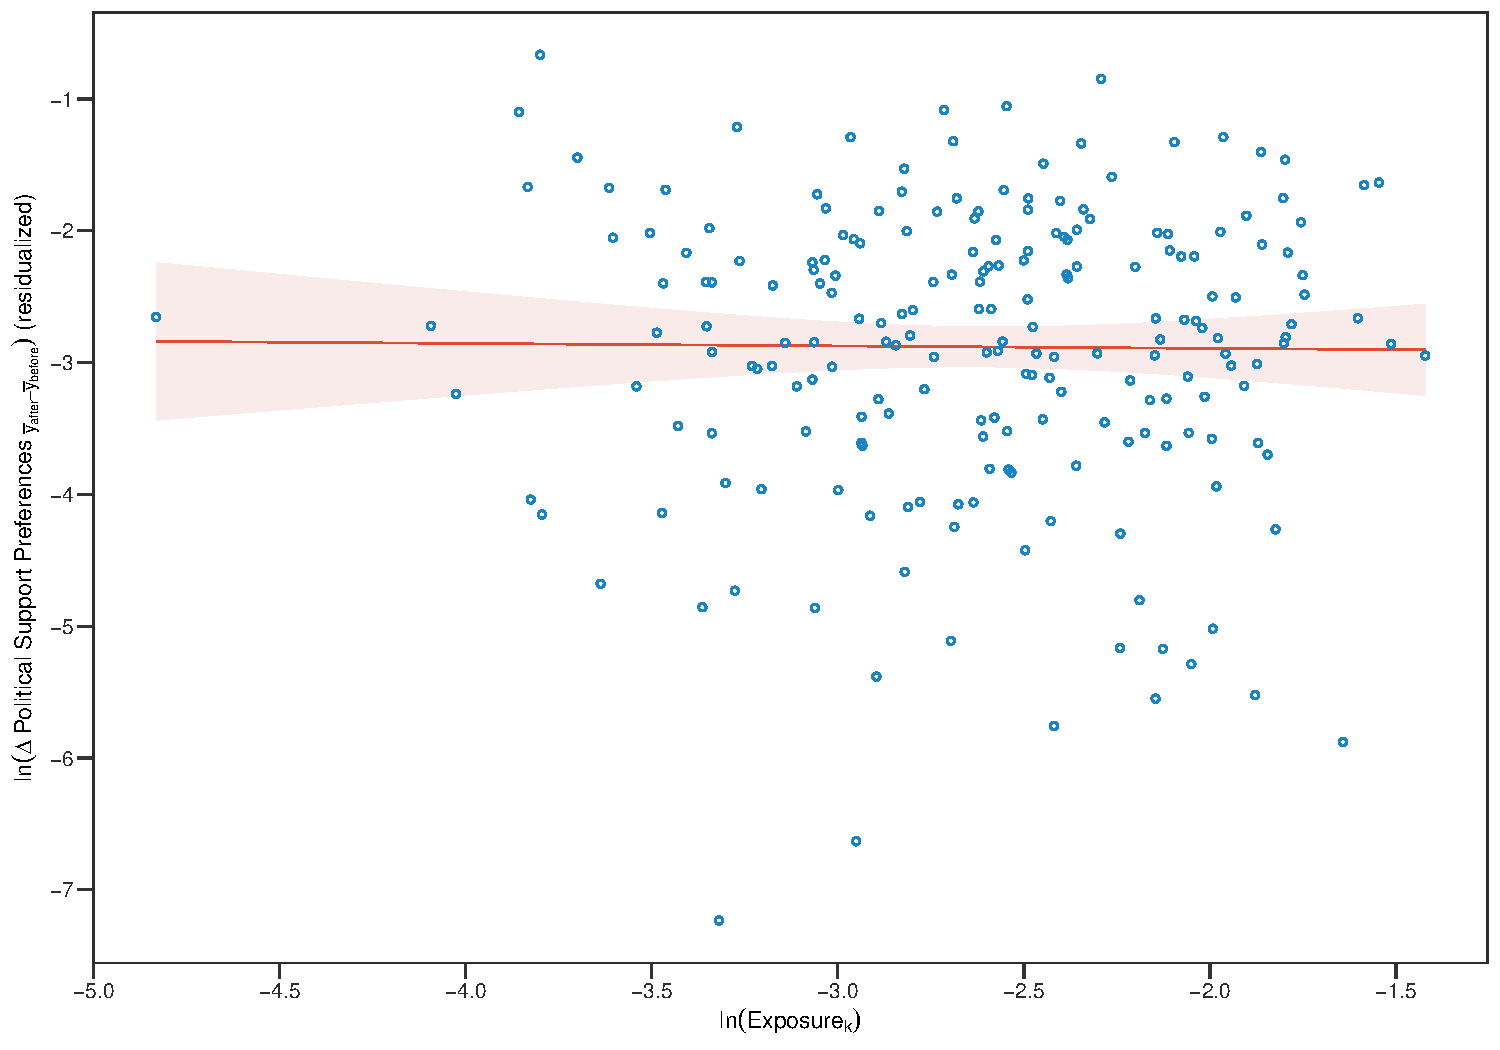
\includegraphics[width=1\linewidth]{heterogeneity/ps_functional_form_cbk_past_mean_noife_logs}
    \begin{tablenotes}
        \footnotesize
        \item \textbf{Notes:}~This table shows ... \hl{XXX}.
    \end{tablenotes} 
\end{figure}

\begin{figure}[htbp!]
    \centering
    \caption{Heterogeneity on Political Support: Continuous Treatment Functional Form (with individual FE) Log-Log}\label{fig:ps_functional_form_cbk_past_mean_ife_logs}
    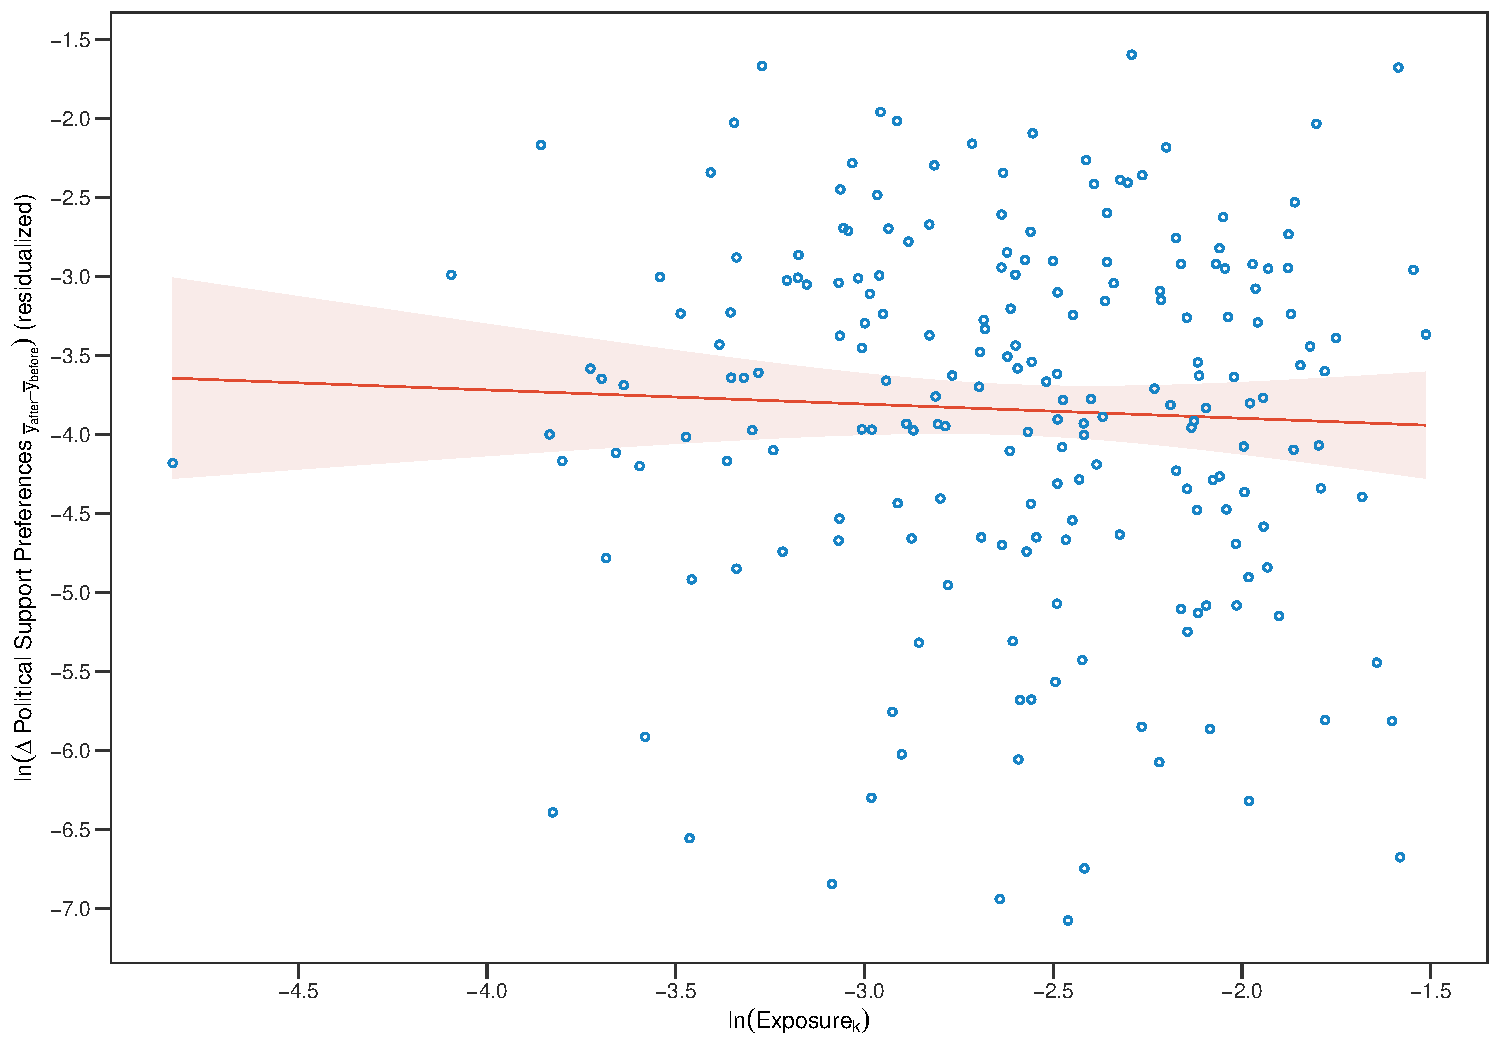
\includegraphics[width=1\linewidth]{heterogeneity/ps_functional_form_cbk_past_mean_ife_logs}
    \begin{tablenotes}
        \footnotesize
        \item \textbf{Notes:}~This table shows ... \hl{XXX}.
    \end{tablenotes} 
\end{figure}

\begin{figure}[htbp!]
    \centering
    \caption{Heterogeneity on Populist Party: Continuous Treatment Functional Form (without individual FE) Log-Log}\label{fig:pp_functional_form_cbk_past_mean_noife_logs}
    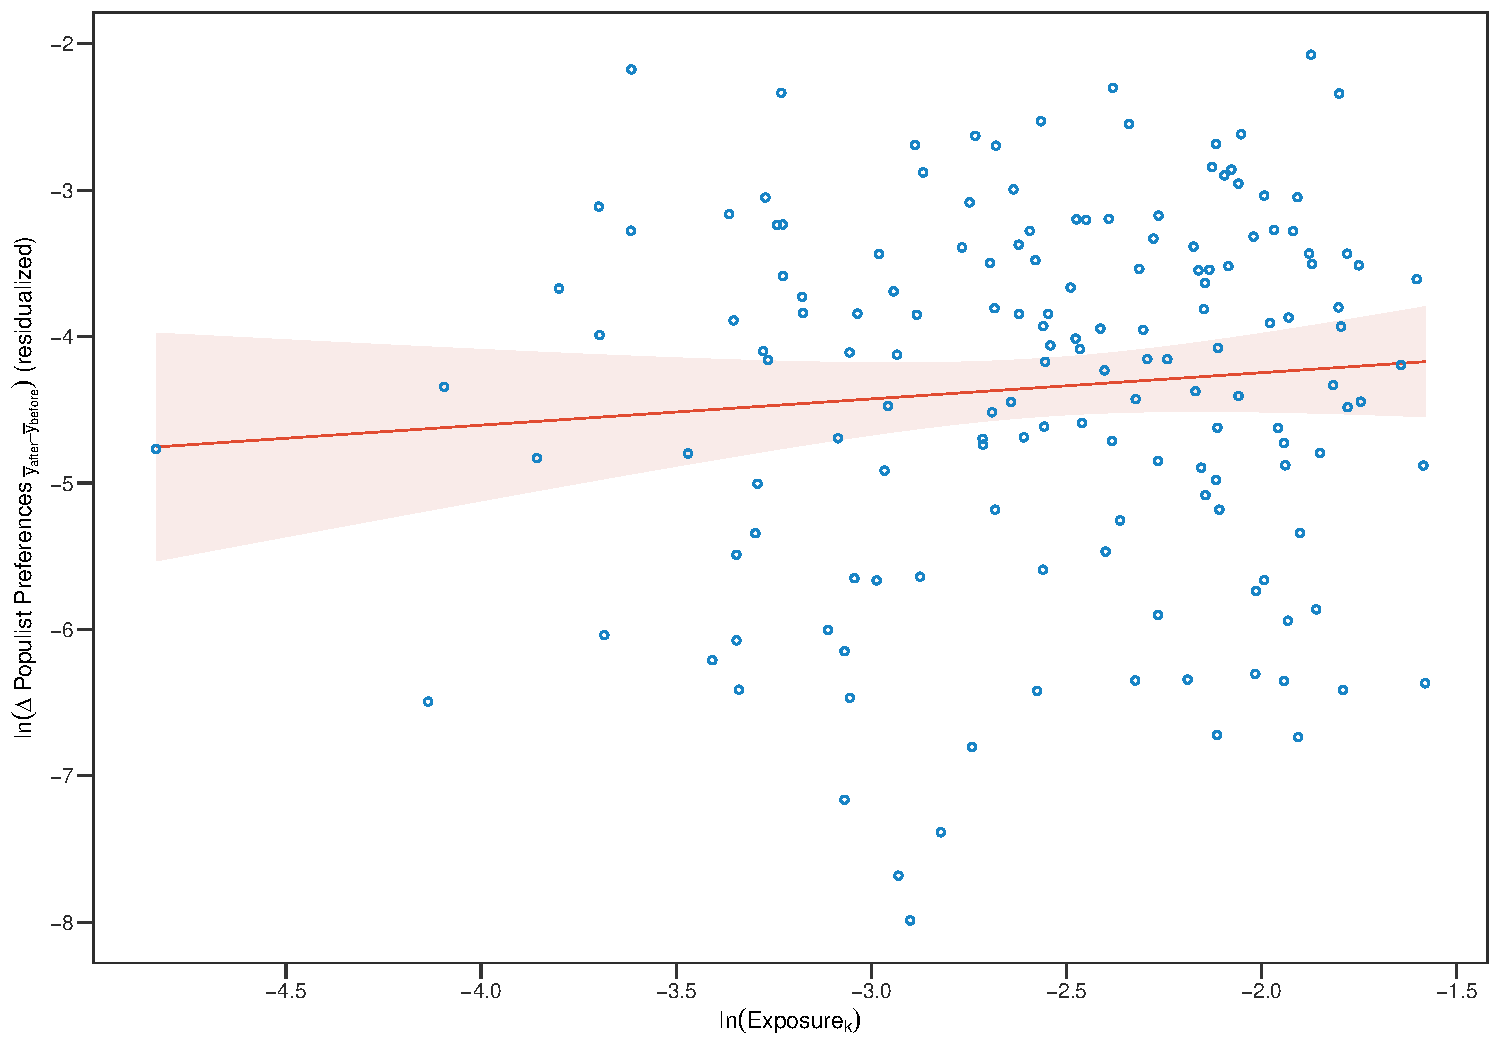
\includegraphics[width=1\linewidth]{heterogeneity/pp_functional_form_cbk_past_mean_noife_logs}
    \begin{tablenotes}
        \footnotesize
        \item \textbf{Notes:}~This table shows ... \hl{XXX}.
    \end{tablenotes} 
\end{figure}

\begin{figure}[htbp!]
    \centering
    \caption{Heterogeneity on Populist Party: Continuous Treatment Functional Form (with individual FE) Log-Log}\label{fig:pp_functional_form_cbk_past_mean_ife_logs}
    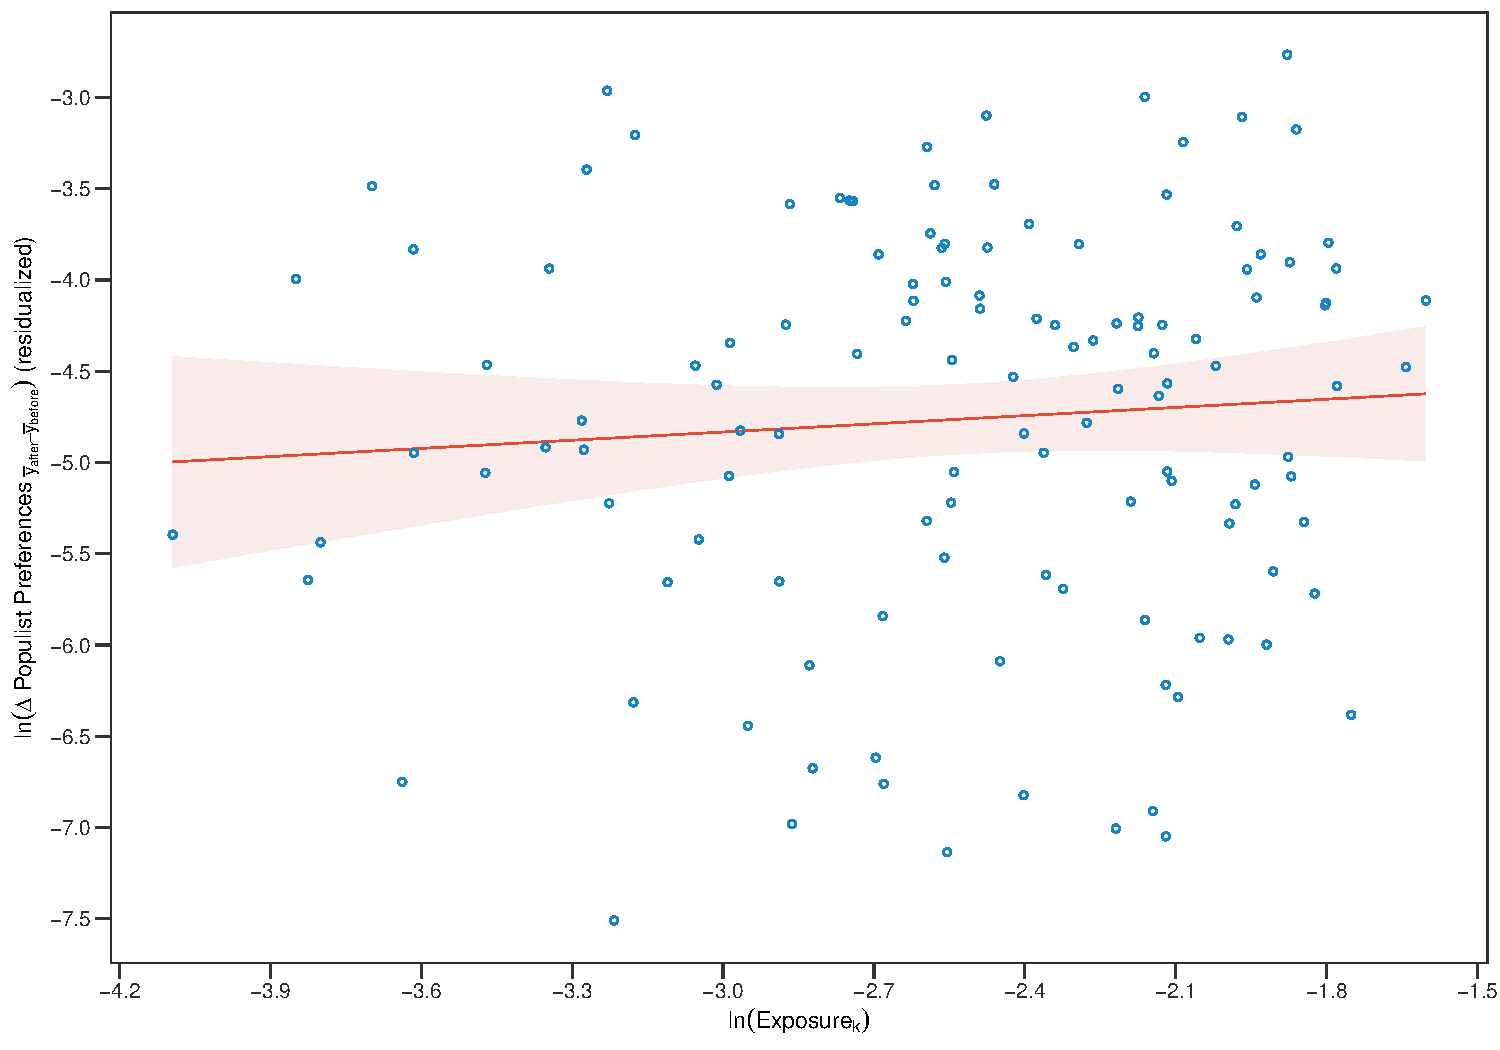
\includegraphics[width=1\linewidth]{heterogeneity/pp_functional_form_cbk_past_mean_ife_logs}
    \begin{tablenotes}
        \footnotesize
        \item \textbf{Notes:}~This table shows ... \hl{XXX}.
    \end{tablenotes} 
\end{figure}

%%%%%%%% OUTCOME TRAJECTORIES

\begin{figure}[htbp!]
    \centering
    \caption{Outcome Trajectories Using Wave Fixed Effects}\label{fig:pp_mean_outcome_cbk_past_mean_p50_sumcoef}
    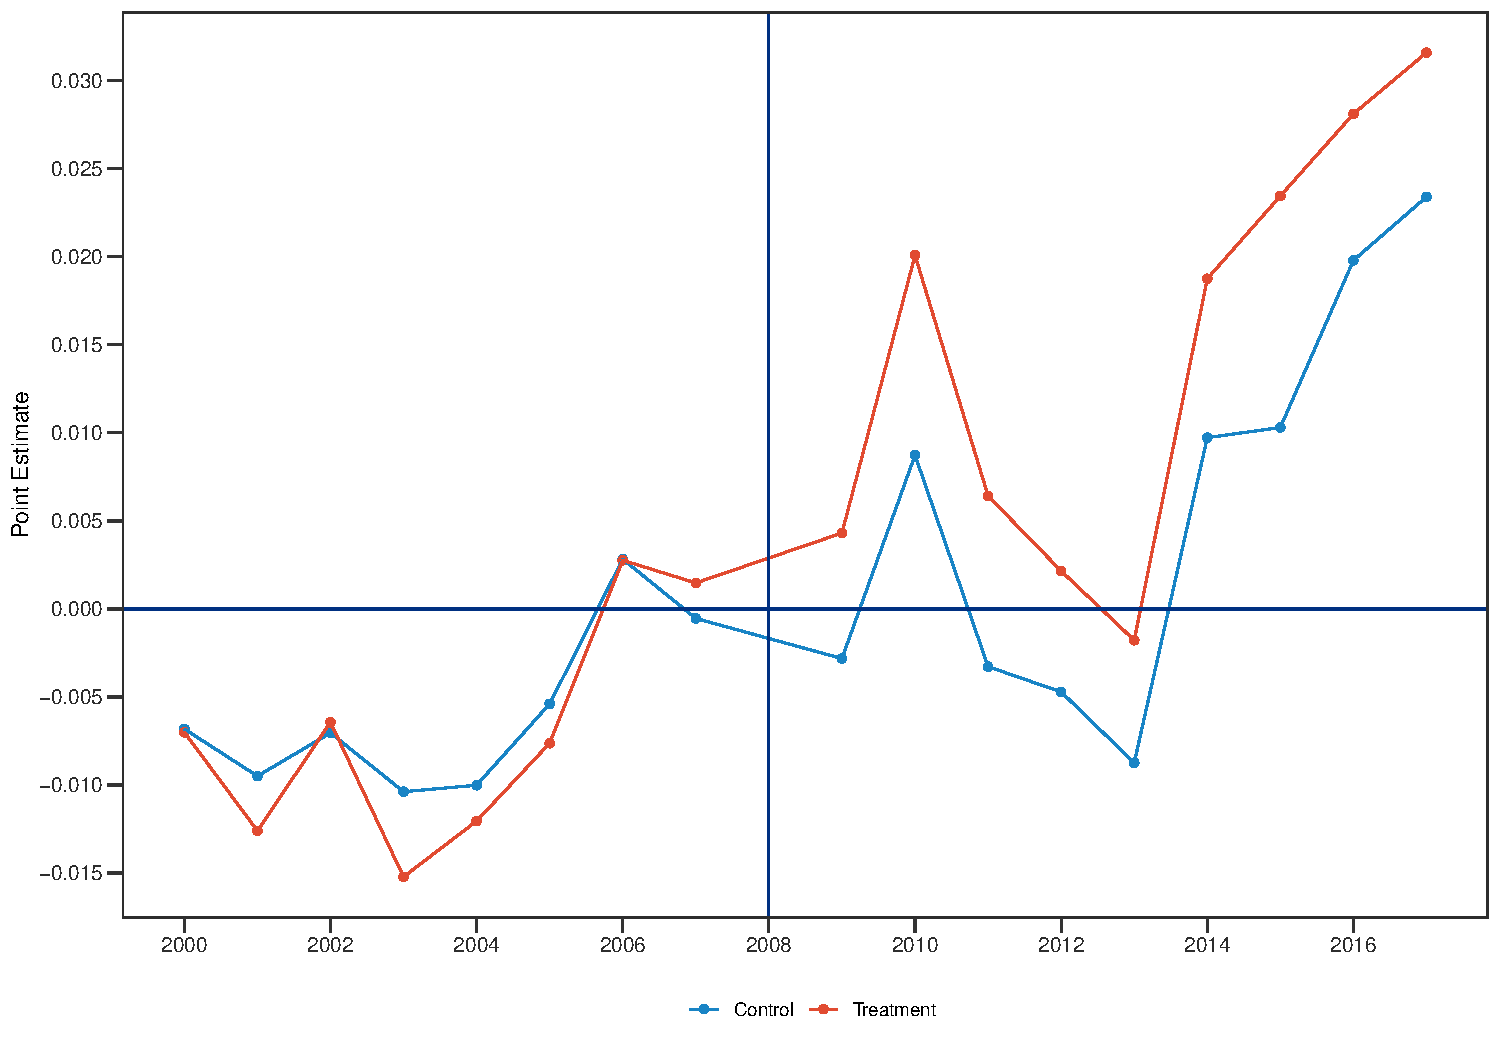
\includegraphics[width=1\linewidth]{events/pp_mean_outcome_cbk_past_mean_p50_sumcoef}
    \begin{tablenotes}
        \footnotesize
        \item \textbf{Notes:}~This table shows ... \hl{XXX}.
    \end{tablenotes} 
\end{figure}

\begin{figure}[htbp!]
    \centering
    \caption{Outcome Trajectories After Residualizing and running regression with dummy for years by treatment group}\label{fig:pp_mean_outcome_cbk_past_mean_p50_noife_allyears}
    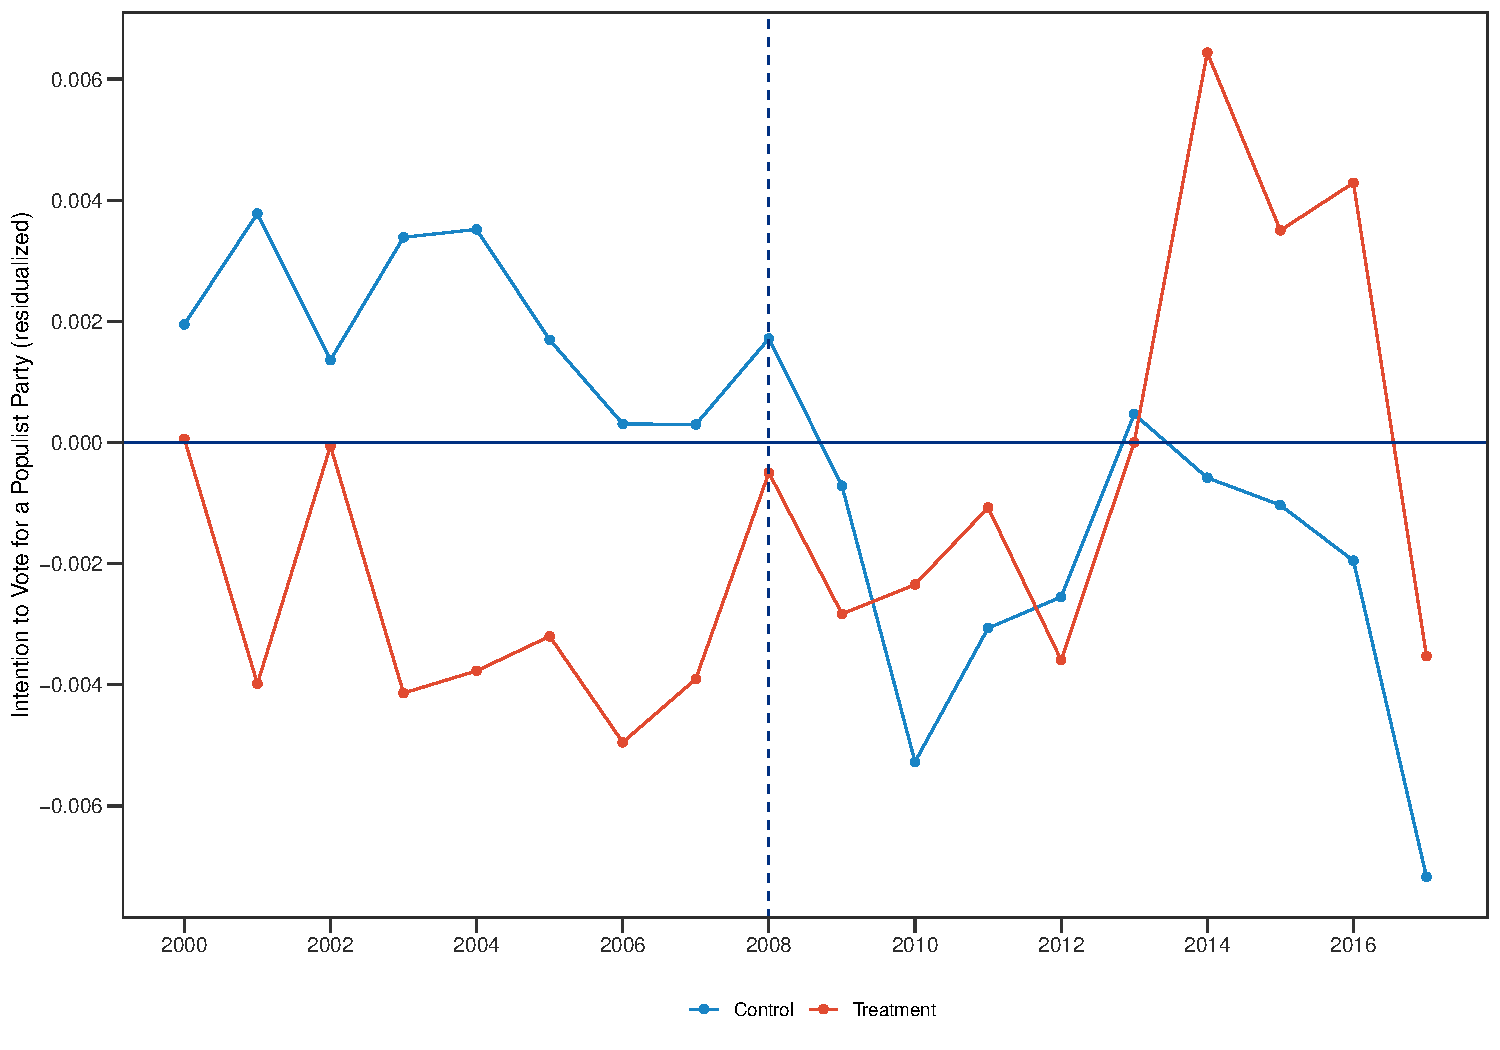
\includegraphics[width=1\linewidth]{events/pp_mean_outcome_cbk_past_mean_p50_noife_allyears}
    \begin{tablenotes}
        \footnotesize
        \item \textbf{Notes:}~This table shows ... \hl{XXX}.
    \end{tablenotes} 
\end{figure}

\begin{figure}[htbp!]
    \centering
    \caption{Outcome Trajectories After Residualizing and running regression with dummy for years by treatment group, reference 2008}\label{fig:pp_mean_outcome_cbk_past_mean_p50_noife}
    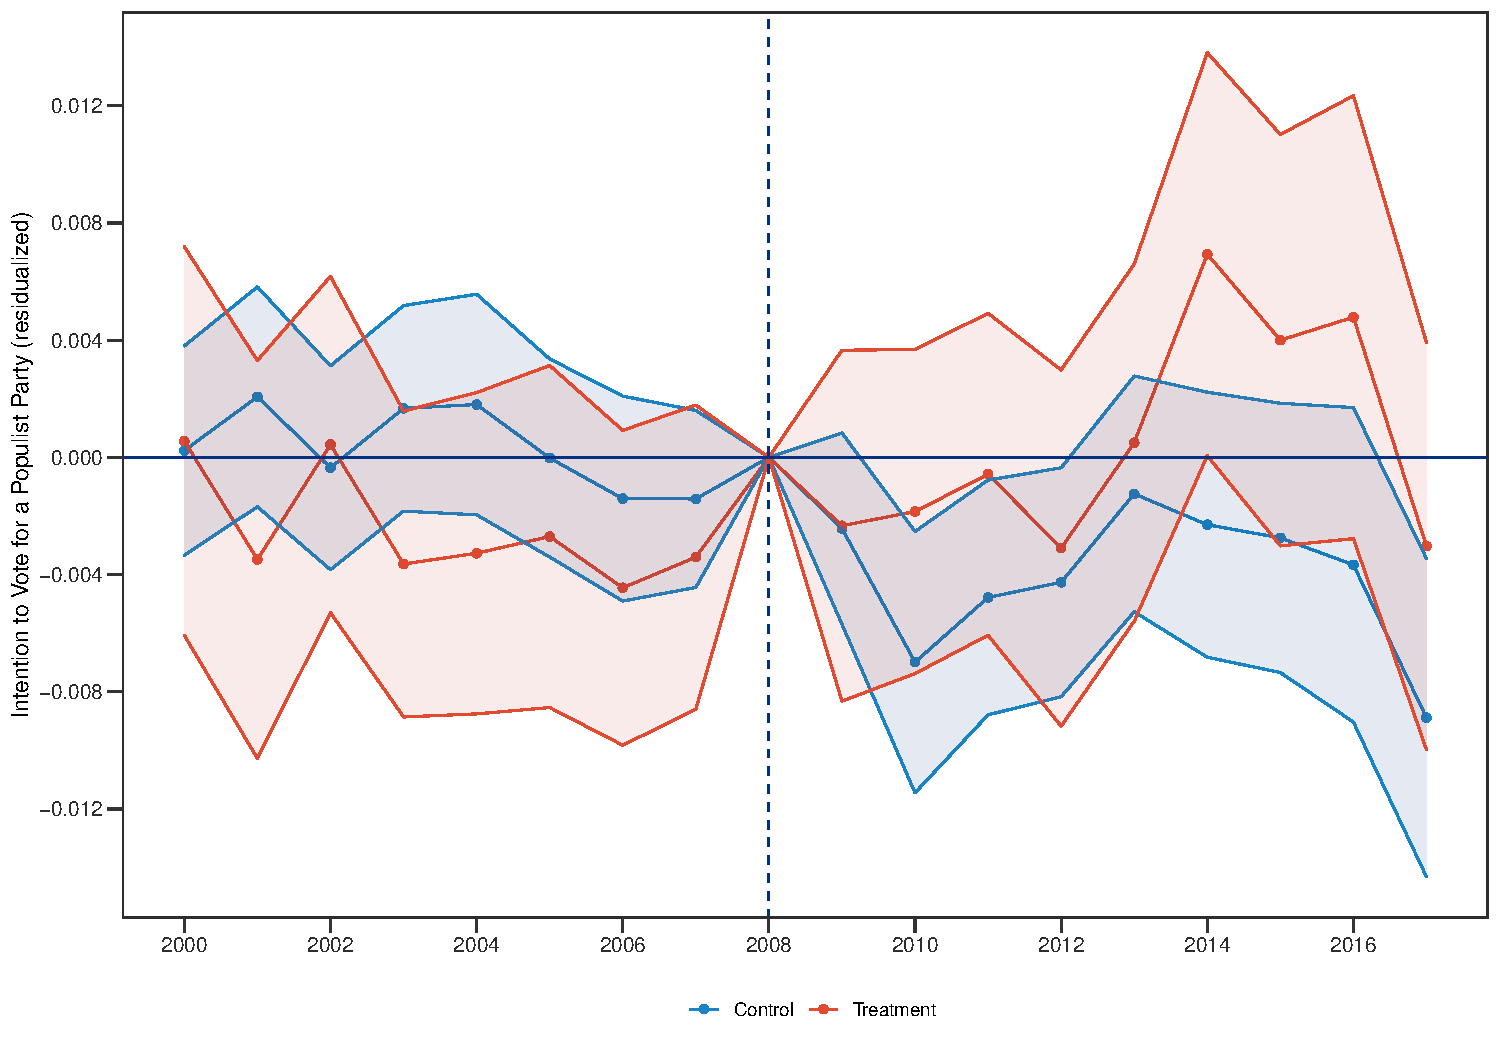
\includegraphics[width=1\linewidth]{events/pp_mean_outcome_cbk_past_mean_p50_noife}
    \begin{tablenotes}
        \footnotesize
        \item \textbf{Notes:}~This table shows ... \hl{XXX}.
    \end{tablenotes} 
\end{figure}


\begin{table}[H]
    \centering
    \caption{The Effect of the Credit Shock on Political Preferences: Outcome as Topic Model Scores}
    \label{tab:rf_text_cbk_past_mean_main_scores}
    \def\sym#1{\ifmmode^{#1}\else\(^{#1}\)\fi}
    \resizebox{\textwidth}{!}{%
        \ExpandableInput{\TablesPath/scores/rf_text_cbk_past_mean_main_scores}
    }%
    \caption*{\footnotesize \textit{Notes:}~This table shows ... \hl{XXX}.}
\end{table}

\begin{table}[H]
     \centering
    \caption{The Effect of the Credit Shock on Political Preferences: Outcome as Dictionary Scores}
    \label{tab:rf_text_cbk_past_mean_main_dict}
    \def\sym#1{\ifmmode^{#1}\else\(^{#1}\)\fi}
        \resizebox{\textwidth}{!}{%
            \ExpandableInput{\TablesPath/scores/rf_text_cbk_past_mean_main_dict}
        }%
    \caption*{\footnotesize \textit{Notes:}~This table shows ... \hl{XXX}.}
\end{table}

%----------------------------------------------------------------------------- %
%   References                                                                 %
%----------------------------------------------------------------------------- %

\clearpage\newpage
\bibliographystyle{aea}
\bibliography{../references/CreditPopulismRefs,../references/ExternalRefs}
% \printbibliography

\end{document}